\chapter{Arquitectura de un robot delta}\label{CAP3}

En este capitulo, se explica detalladamente la descripción del robot delta y las herramientas que se utilizan para la solución de la problemática de la modelación cinemática y dinámica. Inicialmente se explica de forma general el funcionamiento y una estructura básica de un robot delta, con el fin de que el lector de esta tesis entienda lo complejo que es crear un robot por la gran variedad de áreas que lo componen. Luego se muestra y se describen las partes mecánicas o piezas físicas con que esta estructurado. Posteriormente se presenta el funcionamiento y los componentes del middleware ROS, el encargado de controlar y ordenar la lógica de la modelación cinemática y dinámica. Posteriormente se enseña una herramienta de ROS, llamada Rviz, la encargada de la visualización del robot. Finalmente se muestra el sofware que comprueba la modelacion dinamica del sistema, llamado ADAMS.

\section{Funcionamiento general}

La principal tarea de un robot es ir de un punto a otro para realizar determinada acción. Para realizar la tarea se debe pasar por una serie de pasos con el fin de asegurar la ejecución exitosa de dicha tarea. Con el fin de explicar brevemente los pasos a seguir para lograr dicho objetivo, en la figura \ref{f:Cap3-1_diagrama_de_flujo_robot_accion} se muestra un ejemplo básico de un diagrama de flujo de un robot delta accionado por motores paso a paso.\\

Los pasos del diagrama de flujo son los siguientes:

\begin{itemize}
    \item Definir los puntos de inicio y final de la trayectoria del robot.
    \item Elegir el tipo de trayectoria, posiciones, velocidades y aceleraciones impuestas.
    \item Comprobar la cinemática para obtener la trayectoria angular de los motores .
    \item Transformación de la trayectoria cartesiana a la trayectoria en el espacio articular de los actuadores.    
    \item Comprobar dinámica para asegurar que la trayectoria impuesta no dañe los componentes del robot y los motores.
    \item Traducción de trayectoria en el espacio articular a pulsaciones que entiendan los drivers de cada motor.
    \item Envío de pulsos al driver de los motores por medio de un controlador.
    \item Envío de pulsos del driver hacia los motores paso a paso.
\end{itemize}

    \begin{figure}[h]
        \centering
        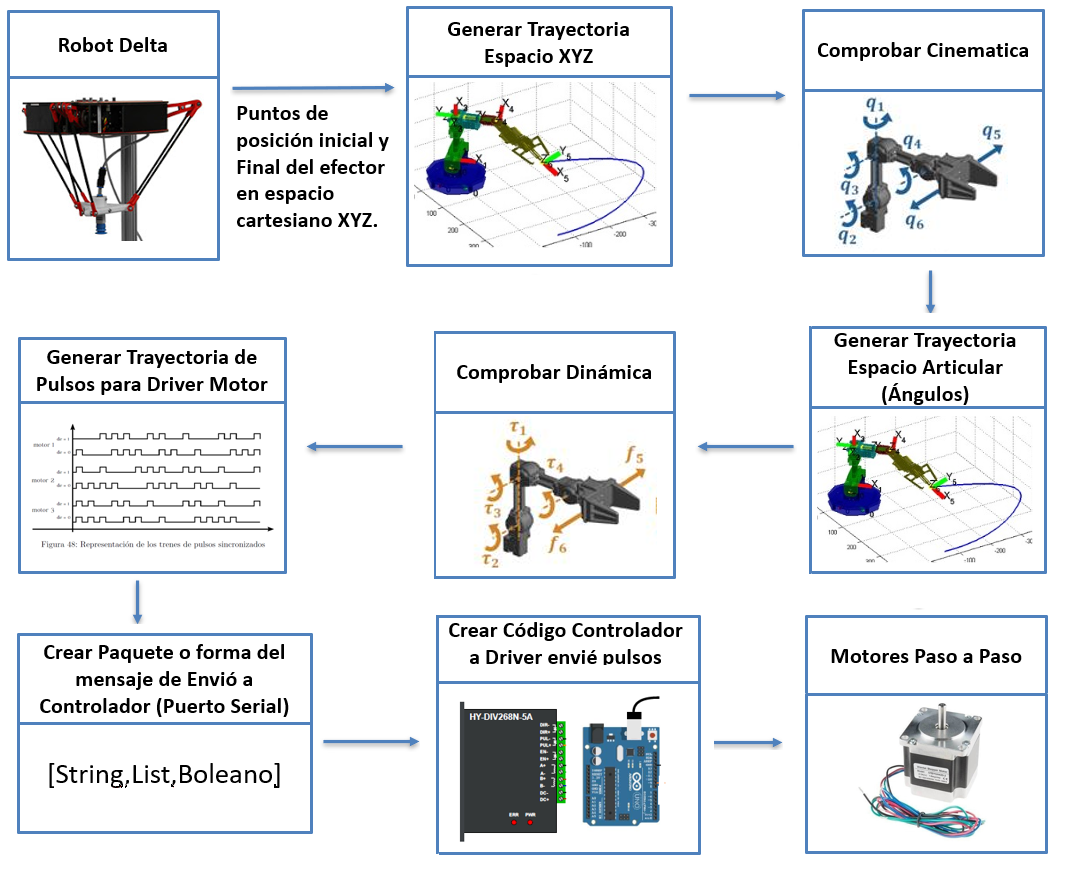
\includegraphics[width=1\linewidth]{Main/Chapter3/Images3/3-1/diagrama-de-flujo-robot.png}
        \caption{Ejemplo de diagrama de flujo de tareas que realiza un robot delta para realizar una trayectoria especifica}
        \label{f:Cap3-1_diagrama_de_flujo_robot_accion}
    \end{figure}
        \newpage
        
\section{Estructura de un robot delta}
%00X0 : reordenar los títulos del cap al diagrama de abajo en formato general, y luego explicar los software específicos para nosotros

    El robot delta puede ser subdivido por categorías de acuerdo al grupo estructural al que pertenezcan. Estas categorías facilitan la generación de conceptos para cada grupo de manera independiente, como se ilustra en la figura \ref{f:Cap3-2_esquema_arquitectura_robot_delta}.
    
    \begin{figure}[h]
        \centering
        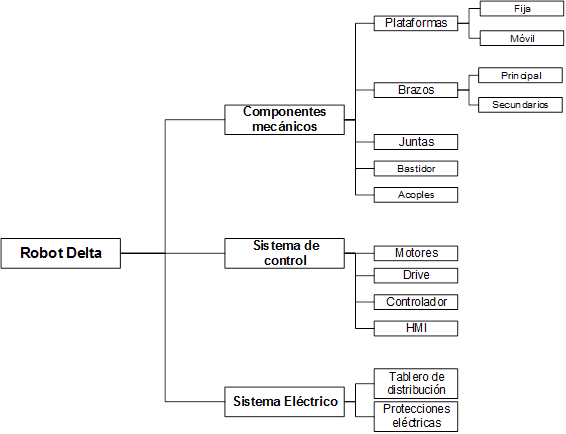
\includegraphics[width=0.85\linewidth]{Main/Chapter3/Images3/3-2/esquema-categorias-estructura.png}
        \caption{Descomposición estructural del robot delta \cite{Robot_parelelo_tipo}}
        \label{f:Cap3-2_esquema_arquitectura_robot_delta}
    \end{figure}
    
    \begin{enumerate}
        \item{ \textbf{Los componentes mecánicos}: son todas las piezas físicas que componen el robot delta. Es muy importante la elección del tipo de juntas a elegir ya que restringen el espacio de trabajo del robot delta. Por otro lado, se pueden optimizar las dimensiones de los largos de los brazos y antebrazos del robot con respecto a la energía suministrada a los motores y al espacio de trabajo.}
        \item{\textbf{El sistema de control}: es todo lo que está relacionado con el control del movimiento del robot delta. Los motores, que mueven los brazos del robot delta, deben controlarse a través de drivers por la complejidad de su accionamiento.}
        \item{ \textbf{El controlador}: puede tener el algoritmo que cree las trayectorias cartesianas para realizar el movimiento del robot de un punto a otro. El HMI es la interfaz que ayuda a visualizar si el movimiento deseado del robot es correcto antes de que se realice.}
        \item{   \textbf{Los componentes eléctricos}: son todo lo relacionado con la electricidad como fuentes de poder para los motores, cables de conexión, fusibles, switch, etc.}
    \end{enumerate}

        \newpage

    Con la intensión de modelar la arquitectura de un robot delta como guía para el desarrollo de este trabajo, se crea una arquitectura con ejemplos reales enfocado solo en el sistema de control, tal como se presenta en la figura \ref{f:Cap3-2_esquema_sistema_control} donde:

    \begin{figure}[h]
        \centering
        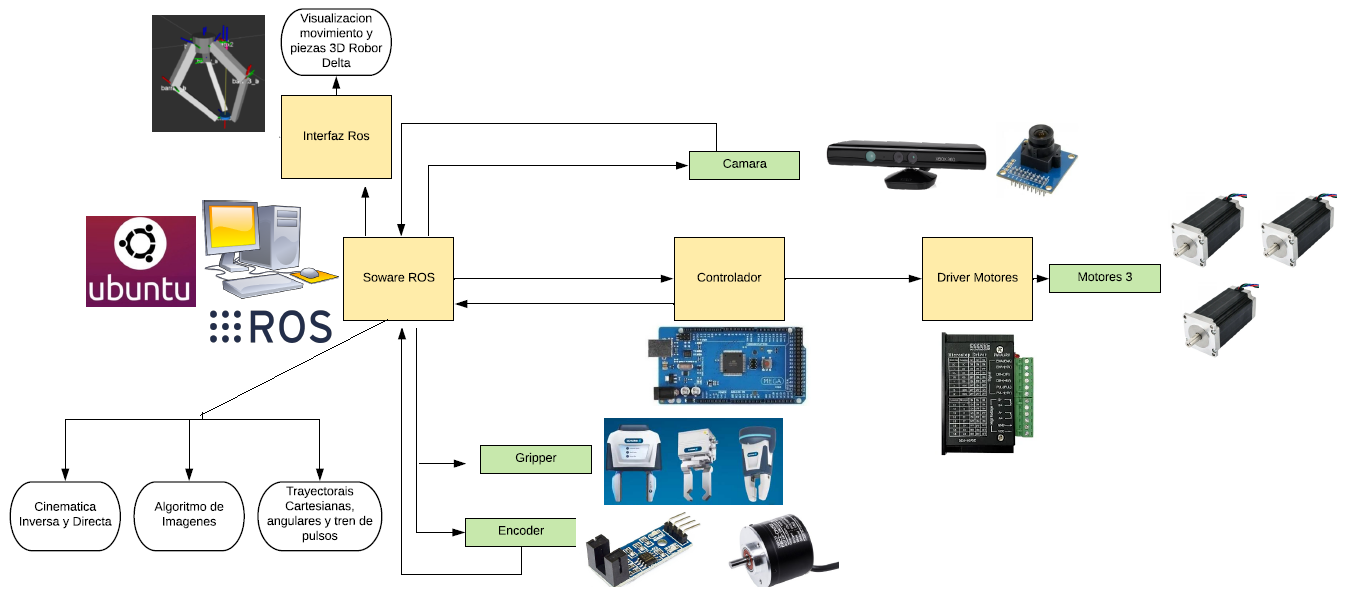
\includegraphics[width=1\linewidth]{Main/Chapter3/Images3/3-2/sistema-de-control.png}
        \caption{Ejemplo de el sistema de control de un robot delta}
        \label{f:Cap3-2_esquema_sistema_control}
    \end{figure}
    
    \begin{itemize}
        \item \textbf{Software ROS:} Es el encargado de procesar y ejecutar los algoritmos de cinemática y dinámica del robot delta. Además, controla el envió, la recepción y el procesamiento de datos de los sensores y el controlador.
        \item \textbf{Controlador:} Realiza la conversión de la trayectoria cartesiana o angular a un formato compatible con el driver de los motores. Se puede utilizar Arduino, Raspberry Pi, etc.
        \item \textbf{Rviz:} Es la interfaz gráfica que simula las trayectorias del robot.
        \item \textbf{Kinect:} Sensor RGB y de profundidad que controla la posición del robot creando un lazo cerrado.
        \item \textbf{Actuadores:} Motores paso a paso controlados por drivers.
        \item \textbf{Encoder:} Sensor de velocidad y posición angular que controla los actuadores creando un lazo cerrado.
        \item \textbf{Gripper:} Pinzas qe sujetan los objetos.
    \end{itemize}
    
    Para controlar a un alto nivel cada punto anterior, se necesita de mucho estudio, investigación y práctica, por lo que en esta tesis solo abarcara lo relacionado con el Software ROS y la interfaz gráfica Rviz.  
    
    \newpage

    
\section{Partes mecánicas}
    Con el fin de describir el robot delta, en esta sección se presenta un resumen del capítulo 2 de la tesis doctoral del ingeniero mecánico Reymond Clavel, el creador de este mecanismo, realizada en École Polytechnique Fédérale de Lausanne \cite{Clavel:31403}. 

    
    \subsection{Investigación}
    El primer objetivo que busca Reymond Clavel es el movimiento de piezas ligeras a gran velocidad en robots, ya que las aplicaciones objetivo de su investigación se encuentran en los campos del envasado en el sector alimentario, despaletización y paletización al inicio o al final de una línea de montaje, el montaje de componentes mecánicos, etc. Para todas estas operaciones se requiere un ritmo alto de producción/operación y los contactos de la industria de Clavel confirmaban esa tendencia en aquellos tiempos.
    
    Para lograr una alta tasa de trabajo durante operaciones que requieren carreras reducidas, el robot debe tener esencialmente una capacidad de aceleración y frenado; esta propiedad se obtiene mediante el uso de potentes actuadores debajo y mediante una estructura móvil muy ligera. Un estudio anterior de robot rápido del Clavel hizo posible probar el uso de gatos hidráulicos a alta velocidad con masas relativamente pesadas, pero por razones de coste y limpieza no querían utilizar energía hidráulica por lo que lo llevo al enfoque de una ``estructura móvil y ligera``.
    
    La búsqueda de un concepto se basó en una metodología enseñada en estudios de microtecnología en EPFL. Según la metodología antes mencionada, el primer paso de la cadena de costos consiste en definir la función global del producto considerado. La representación mediante una caja negra con las diferentes entradas y salidas sintetiza efectivamente esta información.
    
    \begin{figure}[htb]
        \centering
        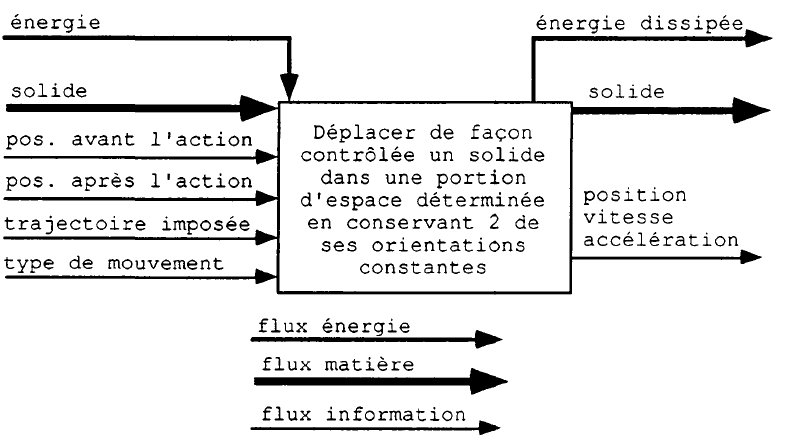
\includegraphics[width=0.75\linewidth]{Main/Chapter3/Images3/3-3/caja-negra-reymond.png}
        \caption{Representación de la función general del robot proyectada en forma de caja negra \cite{Clavel:31403}}
        \label{f:Cap3-3_caja_negra_reymond}
    \end{figure}
    
    \newpage
    
    \subsection{Elección del concepto ``Delta``}
    El catálogo de soluciones del anexo A2.2 de la tesis doctoral \cite{Clavel:31403} presenta 18 tipos de soluciones principales de la estructura de un robot delta que permiten mantener constantes 2 orientaciones de un sólido. La figura \ref{f:Cap3-3_soluciones_interesantes_catalogo} muestra las soluciones más interesantes para el objetivo previsto. 

     \begin{figure}[htb]
        \centering
        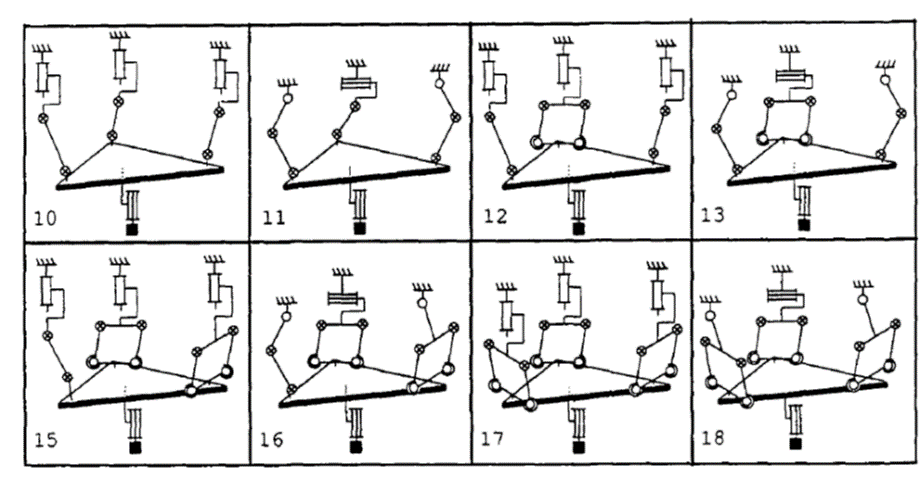
\includegraphics[width=0.85\linewidth]{Main/Chapter3/Images3/3-3/soluciones-interesantes.png}
        \caption{Extracto de las soluciones del catálogo del Apéndice A.2.2  \cite{Clavel:31403}}
        \label{f:Cap3-3_soluciones_interesantes_catalogo}
    \end{figure}
 
      \begin{figure}[htb]
        \centering
        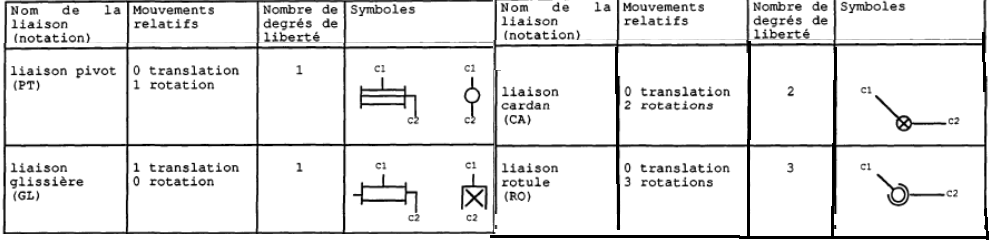
\includegraphics[width=0.8\linewidth]{Main/Chapter4/Images4/juntas.png}
        \caption{Nombre, movimiento relativo. grados de libertad y simbolos de juntas dibujadas en la figura  \ref{f:Cap3-3_soluciones_interesantes_catalogo}  \cite{Clavel:31403}}
        \label{f:Cap3-3_soluciones_interesantes_catalogo_JUNTAS}
    \end{figure}
 
 Entre estas 18 soluciones, Reymond conserva aquellas que tienen las siguientes particularidades:   
    \begin{itemize}
        \item El movimiento en el espacio (con tres grados de libertad) es proporcionado por el tres actuadores asegurados a la base fija, las soluciones 10 a 13 y 15 a 18 de la figura \ref{f:Cap3-3_soluciones_interesantes_catalogo} cumplen esta condición.
        \item Los actuadores son del tipo giratorio. Las soluciones 11, 13, 16 y 18 cumplen esta condicion.
        \item La estabilidad del órgano terminal está asegurada por una mayoría de elementos que trabajan en tensión-compresión más que en torsión. Finalmente se adopta la solución numero 18.
    \end{itemize}
    

    
        \newpage
    
    \subsection{Descripción del concepto ``Delta'' y sus componentes}
    La figura \ref{f:Cap3-3_esquema_principal_robot_delta} sirve de apoyo para la descripción del robot Delta y su funcionamiento. Este es un robot con cuatro grados de libertad. Se compone principalmente de una ``base fija'' (1) integrada a un marco de soporte de la instalación y una placa móvil (5); el nombre que se le da a esta última pieza es ``góndola'' (nacelle en frances). La conexión entre la base fija (1) y la góndola (5) se realiza mediante tres cadenas cinemáticas, cada una de ellas está formado por un ``brazo'' (2) montado en una articulación pivotante sobre la base fija y 2 ``barras paralelas'' (3) provistas cada una de una articulación (4) en cada extremo. El conjunto anterior que forma 2 barras paralelas y 2 elementos de conexión al brazo y a la góndola, se denomina ``paralelogramo''. Cada brazo (2) es impulsado por un ``motor de brazo'' (7) que, con mayor frecuencia, adopta la forma de un conjunto de motor reductor de sensor. La ``Pinza'' (10) del motor (6), a través del ``eje telescópico'' (8) provisto de una articulación tipo cardan (9) tiene oculto uno de sus extremos.

    \vspace{-1em}

    % Multiples imagenes        
    \begin{figure}[h]
         \centering
              \subfloat[Esquema principal del robot delta]{
               \label{f:Cap3-3_esquema_principal_robot_delta}
                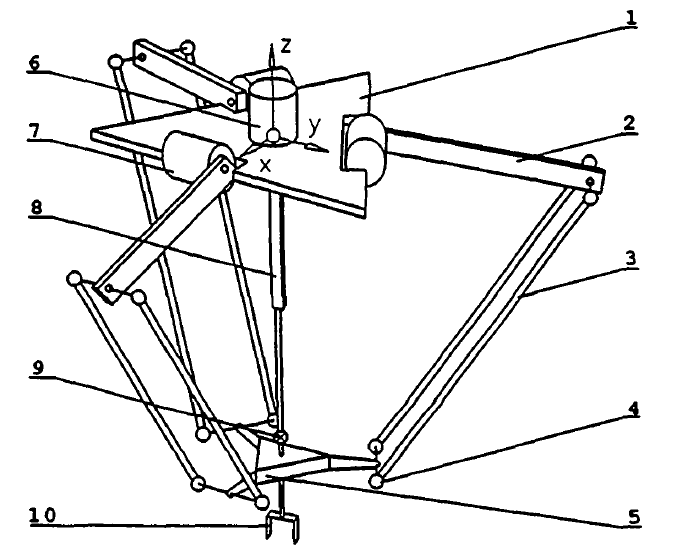
\includegraphics[width=0.5\textwidth]{Main/Chapter3/Images3/3-3/esquema-principal-robot-delta.png}}
              \subfloat[Representación de paralelogramos del robot delta]{
               \label{f:Cap3-3_ayuda_dimensiones}
                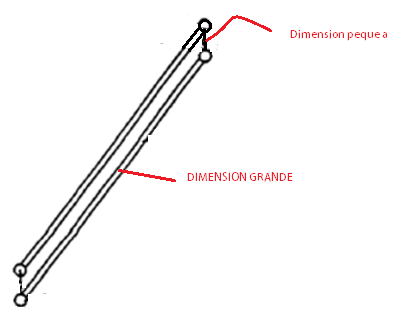
\includegraphics[width=0.5\textwidth]{Main/Chapter3/Images3/3-3/ayuda-dimensiones.png}}
         \caption{Descripción visual de un robot delta \cite{Clavel:31403}}
         %\label{f:animales}
    \end{figure}

    La orientación de la góndola está asegurada constantemente por los 3 paralelogramos (figura \ref{f:Cap3-3_ayuda_dimensiones}), que comprenden cada uno 2 dimensiones pequeñas y 2 dimensiones grandes formadas por las barras paralelas. Cada lado pequeño integrado al extremo de un brazo permanece constantemente paralelo al eje de rotación del brazo en cuestión. Los 3 pares de barras paralelas aseguran que las 3 pequeñas dimensiones integradas a la góndola permanezcan paralelas a las pequeñas dimensiones integradas a los extremos de los brazos, por tanto, paralelas a los ejes de rotación de los brazos que, por construcción, se ubican en el mismo plano. Las juntas en los extremos de las barras paralelas son del tipo de junta esférica, por lo que cada barra puede girar alrededor de su eje longitudinal; esta rotación no altera el comportamiento de esta estructura articulada que forma el paralelogramo del espacio. Una conexión por resortes y estribos entre las 2 barras paralelas simplifica la construcción de las rótulas.
    
    \newpage

\section{Software Robor Operating System (ROS)}
    
        En esta sección se proporciona una descripción general de Robot Operating System, por sus siglas ROS y sus principales lineamientos. ROS es un marco para desarrollar software de robótica. El software está estructurado bajo un paradigma modular, pequeños paquetes que se comunican entre si mediante rápidos mensajes. Este paradigma se fomenta la reutilización de código y la colaboración global por sobre los entornos particulares.
    
    \begin{figure}[htb]
        \centering
        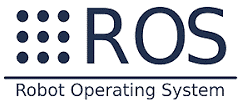
\includegraphics[width=0.5\linewidth]{Main/Chapter3/Images3/3-4/logo-ros.png}
        \caption{Logo de ROS \cite{ros2222}}
        \label{f:Cap3-4_logo_ros}
    \end{figure}
    
    \subsection{Historia}
    
        ROS es un gran proyecto que tiene muchos antepasados y contribuyentes. Mucha gente en la comunidad de investigación robótica sintió la necesidad de un marco de colaboración abierto. Varios proyectos en la Universidad de Stanford (figura \ref{f:Cap3-4_entidades_inicio_ros_32}) a mediados de la década de 2000 involucraban inteligencia artificial incorporada e integradora, como el Stanford AI Robot (STAIR) y el programa Personal Robots (PR), que crearon prototipos internos de los tipos de sistemas de software dinámicos y flexibles como lo es ROS. Se basó en Switchyard, que era parte de un proyecto de STAIR y fue escrito por Morgan Quigley en Stanford. En 2007, Willow Garage, Inc., una incubadora de robótica cercana, proporcionó importantes recursos para extender estos conceptos mucho más y crear implementaciones bien probadas. Desde el 2013 hasta el presente, ROS es mantenido permanentemente por Open Source Robotics Foundation (OSRF, figura \ref{f:Cap3-4_entidades_inicio_ros_334}) de Google y desde el 2017 cambio su nombre a Open Robotics.
        
        \begin{figure}[htbp]
            \centering
            
\includegraphics[width=0.7\linewidth]{Main/Chapter3/Images3/3-4/entidade-asociadas-al-inicio-de-ros-3.png}
            \caption{OSRF \cite{osrf}} 
            \label{f:Cap3-4_entidades_inicio_ros_334}
        \end{figure}        
        
        \newpage
        
        La mayoría de las compañías y laboratorios de investigación en robótica están ahora portando su software a ROS. Esta tendencia también es visible en robots industriales, donde compañías están paulatinamente migrando de aplicaciones propietarias a ROS. El movimiento llamado ROS Industrial se ha incrementado en estos últimos años y su objetivo, básicamente, consiste en extender las capacidades avanzadas de ROS a la automatización y la robótica industrial. Este proyecto comenzó como un intento de colaboración de Yaskawa Motoman Robotics, Southwest Research Institute (SwRI) y Willow Garage (figura \ref{f:Cap3-4_entidades_inicio_ros_33364}). En enero de 2012, Shaun Edwards de SwRI fundó un software repositorio, alojado en Github, donde la comunidad robótica puede encontrar interfaces para manipuladores industriales, pinzas, sensores y redes de dispositivos.
        
        \begin{figure}[htbp]
            \centering
            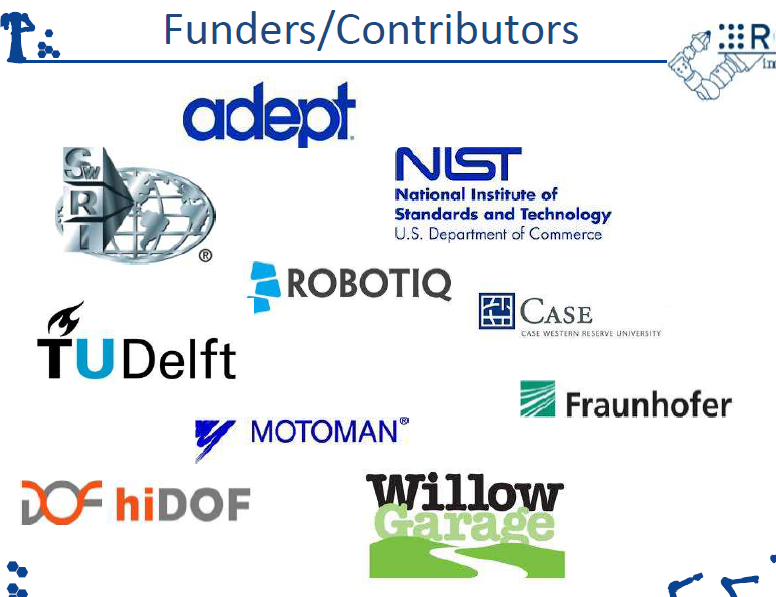
\includegraphics[width=0.65\linewidth]{Main/Chapter3/Images3/3-4/entidade-asociadas-al-inicio-de-ros-2.png}
            \caption{Fundadores y contribuidores de ROS} 
            \label{f:Cap3-4_entidades_inicio_ros_33364}
        \end{figure}    
        
        Finalizando con la breve historia de ROS, se puede decir que se utiliza en estos momentos en todo el mundo en instituciones académicas, industriales y de investigación. Los desarrolladores han contribuido con miles de paquetes, incluidas soluciones de algunos de los principales expertos del mundo en áreas específicas. Las nuevas empresas de robots ofrecen interfaces ROS con sus productos, y las empresas de robots industriales establecidas también están introduciendo interfaces ROS. Con la adopción generalizada de ROS como el enfoque estándar de factor para la programación de robots, existe una nueva esperanza de acelerar las capacidades de los robots.
        
        \begin{figure}[htbp]
            \centering
            
\includegraphics[width=0.6\linewidth]{Main/Chapter3/Images3/Stanford-University-logo1.jpg}
            \caption{Logo Stanford University \cite{stanford}} 
            \label{f:Cap3-4_entidades_inicio_ros_32}
        \end{figure}

    \newpage

    \subsection{Problema Principal}
    
    La intención con que se creó ROS fue de permitir a los investigadores desarrollar rápidamente nuevos sistemas robóticos sin tener que reinventar todo nuevamente, mediante el uso de herramientas e interfaces estándar. Para hacer más eficientes los procesos de investigación y desarrollo de software de robots, se detectaron los siguientes 3 problemas a solucionar:
    
    \begin{itemize}
        \item {Programación secuencial inadecuada para el mundo asincrónico robótico (figura \ref{f:Cap3-4_entidades_ini_ros_1})}
        \item {Sistemas robóticos deben gestionar una complejidad significativa}
        \item {Abstracción de los detalles de un hardware específico del robot.}
    \end{itemize}

        \begin{figure}[htbp]
            \centering
            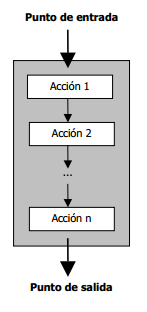
\includegraphics[width=0.25\linewidth]{Main/Chapter3/Images3/agrupar_problem_111.png}
            \caption{Programación Secuencial}
            \label{f:Cap3-4_entidades_ini_ros_1}
        \end{figure}
        
    La solución para el problema de programación secuencias se basó en Callback, que son una función que se ejecuta siempre que hay datos disponibles para su procesamiento. Son asincrónico, ya que la devolución de llamada puede ocurrir en cualquier momento. Con respecto a el problema de softwares multifuncionales complejos y atracción de detalles de hardware específicos, se separaron los procesos en “nodos” que se comunican a través de una interfaz de mensajería. Por ejemplo, se separaron los procesos de las cámaras, edometría, escáner láser y creación de mapas y estos interactúan a través de una interfaz que comunica estos procesos por medio de “temas”. Estos últimos conceptos se explican en detalle en secciones posteriores.

    \newpage


    \subsection{Que es ROS}
       ROS es una abreviatura de  Robot Operating System y es una plataforma de desarrollo de aplicaciones en robótica que provee estilos de programación (en particular, que se basa en nodos distribuidos y acoplados libremente); definiciones de interfaz y paradigmas para las comunicaciones entre nodos ; definiciones de interfaz para la incorporación de bibliotecas y paquetes; una colección de herramientas para visualización, depuración, registro de datos y diagnóstico del sistema; un repositorio de código fuente compartido; y puentes a múltiples bibliotecas útiles e independientes de código abierto.
       
       El objetivo principal de ROS es apoyar la reutilización de código en la investigación y el desarrollo de robótica. ROS es un marco distribuido de procesos (también conocido como nodos) que permite que los ejecutables se diseñen individualmente y se acoplen libremente en tiempo de ejecución. Estos procesos se pueden agrupar en paquetes, que se pueden compartir y distribuir fácilmente. ROS también es compatible con un sistema federado de repositorios de código que también permite la distribución de la colaboración. Este diseño, desde el nivel del sistema de archivos hasta el nivel de la comunidad, permite decisiones independientes sobre el desarrollo y la implementación, pero todos pueden combinarse con las herramientas de infraestructura ROS.
       
       ROS no es un sistema operativo convencional como Windows, Linux y Android en el sentido tradicional de gestión y programación de procesos; más bien, es un meta-sistema operativo que se ejecuta en el sistema operativo. Las diferencias entre un OS y ROS se muestran el la figura \ref{f:Cap3-4_diferencias_ros_so}. ROS es un middleware, que proporciona los servicios que esperaría de un sistema operativo, incluida la abstracción de hardware, control de dispositivos de bajo nivel, implementación de funciones de uso común, transmisión de mensajes entre procesos y administración de paquetes. También proporciona herramientas y bibliotecas para obtener, compilar, escribir y ejecutar código en varios equipos.
       
        \begin{figure}[htb]
            \centering
            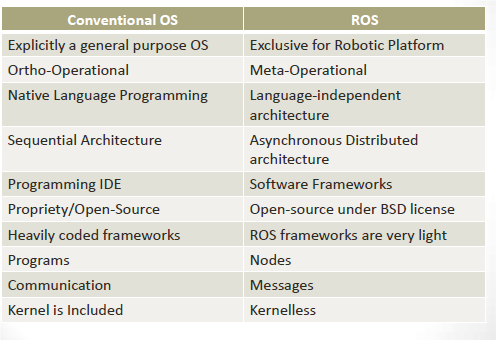
\includegraphics[width=0.65\linewidth]{Main/Chapter3/Images3/3-4/diferencia-ROS-SO.png}
            \caption{Diferencias entre un sistema operativo convencional y ROS}
            \label{f:Cap3-4_diferencias_ros_so}
        \end{figure}
        
        \newpage
        
        Las principales características de ROS se pueden resumir de la siguiente manera:
        
        \begin{itemize}
            \item \textbf{Plumbing:} ROS proporciona una infraestructura de mensajería de publicación y suscripción diseñada para respaldar la construcción rápida y sencilla de sistemas informáticos distribuidos.
            \item \textbf{Herramientas} ROS proporciona un amplio conjunto de herramientas para configurar, iniciar, introspectar, depurar, visualizar, registrar, probar y detener sistemas informáticos distribuidos.
            \item \textbf{Capacidades} ROS proporciona una amplia colección de bibliotecas que implementan funcionalidades robóticas útiles, con un enfoque en la movilidad, la manipulación y la percepción.
            \item \textbf{Ecosistema:} ROS es apoyado y mejorado por una gran comunidad, con un fuerte enfoque en la integración y documentación. ros.org es una ventanilla única que busca y aprende sobre los miles de paquetes ROS que están disponibles a través de desarrolladores de todo el mundo.
        \end{itemize}

        Un ejemplo se muestra en la figura \ref{f:Cap3-4_compatibilidad_ros}, la comunicación de datos ROS es compatible no solo con un sistema operativo, sino también con múltiples sistemas operativos, hardware y programas, lo que lo hace muy adecuado para el desarrollo de robots donde se combinan varios hardware. 
        
        \begin{figure}[htb]
            \centering
            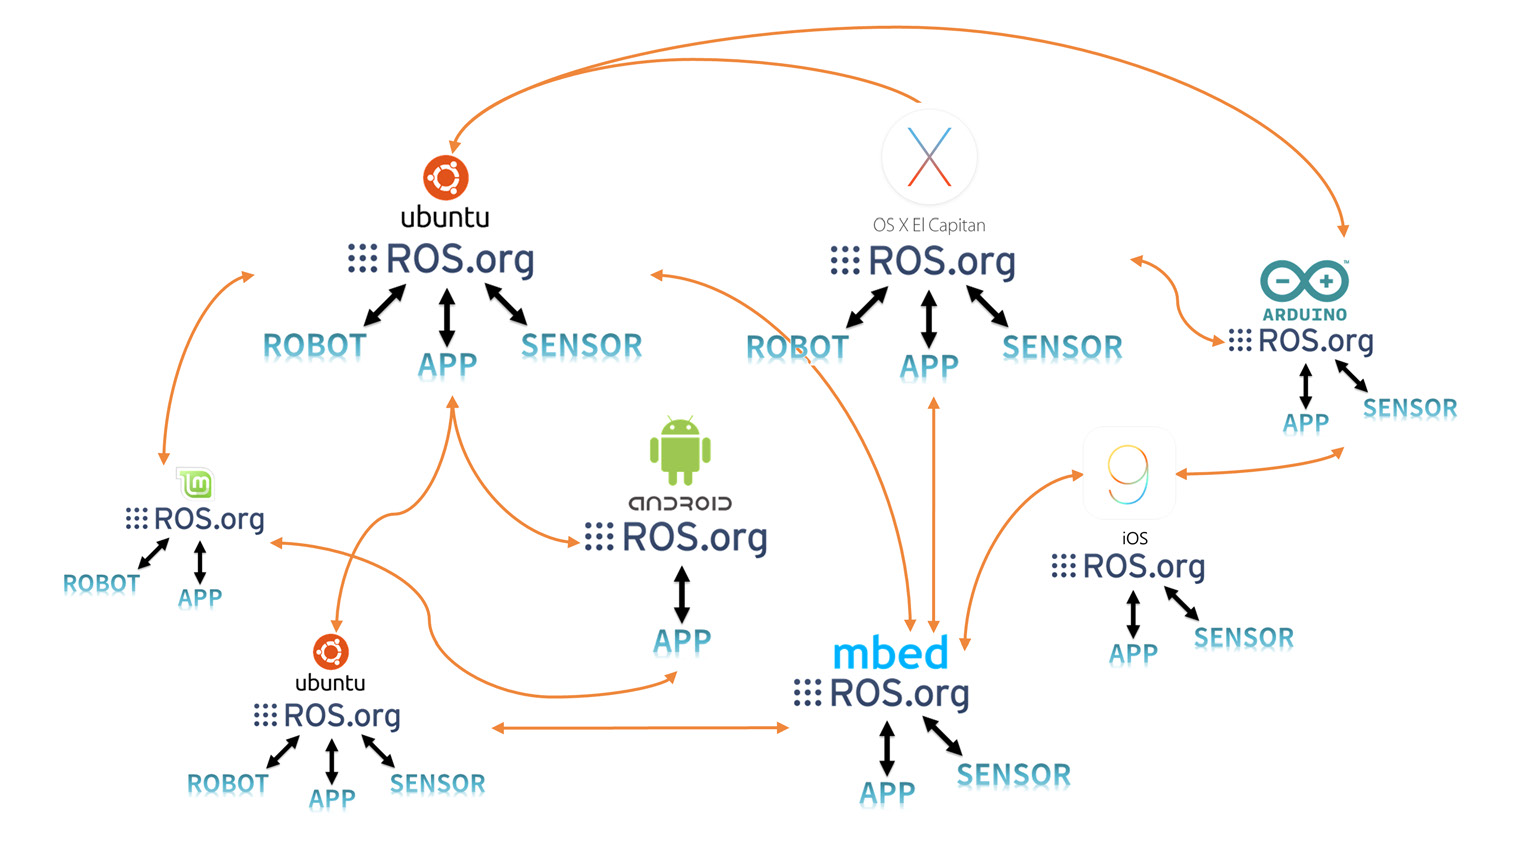
\includegraphics[width=1.0\linewidth]{Main/Chapter3/Images3/3-4/compatibilidad-ros.png}
            \caption{Compatibilidad de ROS y otras plataformas \cite{ROS_BOOK_1}}
            \label{f:Cap3-4_compatibilidad_ros}
        \end{figure}
        
    \newpage

        
    \subsection{Objetivos de ROS}
    
        Todos los marcos de software imponen sus filosofías de desarrollo a sus colaboradores directa o indirectamente, a través de sus modismos y prácticas comunes. En términos generales, ROS sigue la filosofía de desarrollo de software de Unix en varios aspectos clave. Esto tiende a hacer que ROS se sienta ``natural'' para los desarrolladores que provienen de Unix, pero algo ``críptico'' al principio para aquellos que han utilizado principalmente entornos de desarrollo gráfico en Windows o Mac OS X. Los siguientes párrafos describen varios aspectos filosóficos de ROS.
        
        \subsubsection{Peer to peer (Nodos)}
        
            Los sistemas ROS consisten en numerosos programas pequeños de computadora que se conectan entre sí e intercambian mensajes continuamente. Estos mensajes viajan directamente de un programa a otro; no hay un servicio de enrutamiento central. Aunque esto hace que la ``plumbing'' subyacente sea más compleja, el resultado es un sistema que escala mejor a medida que aumenta la cantidad de datos. La mentalidad Peer to peer se representa en la figura \ref{f:Cap3-5_arquitectura_ros}.
            
            \begin{figure}[htb]
                \centering
                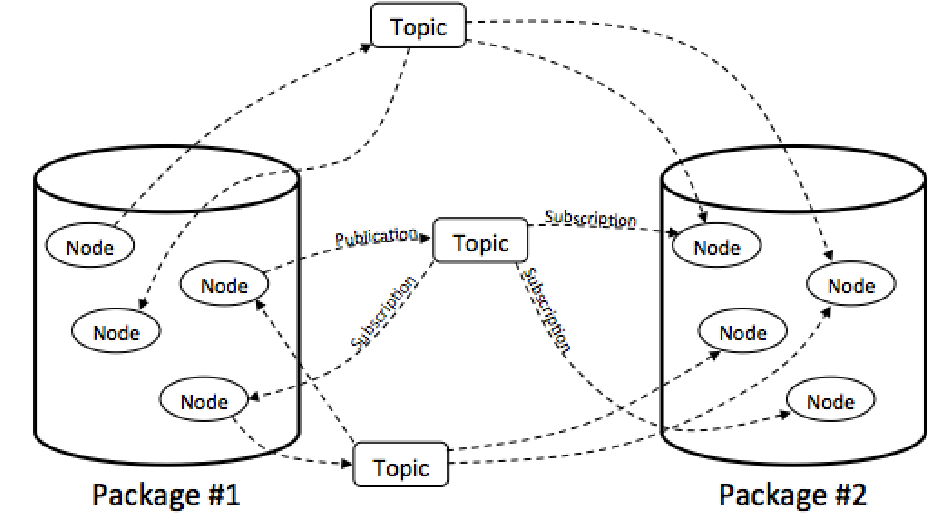
\includegraphics[width=0.8\linewidth]{Main/Chapter3/Images3/arquitectura_por_nodos_1.png}
                \caption{Modelo de cómo los nodos ROS publican y se suscriben a temas \cite{naval_delta}}
                \label{f:Cap3-5_arquitectura_ros}
            \end{figure}
            
        \subsubsection{Orientación hacia las herramientas}
        
            Como lo demuestra la arquitectura duradera de Unix, se pueden crear sistemas de software complejos a partir de muchos programas pequeños y genéricos. A diferencia de muchos otros marcos de software de robótica, ROS no tiene un entorno de ejecución y desarrollo integrado canónico. Tareas como navegar por el árbol del código fuente, visualizar las interconexiones del sistema, trazar gráficamente los flujos de datos, generar documentación, registrar datos, etc, son todas realizadas por programas separados. Esto fomenta la creación de implementaciones nuevas y mejoradas, ya que (idealmente) se pueden intercambiar por implementaciones más adecuadas para un dominio de tarea en particular. Las versiones recientes de ROS permiten que muchas de estas herramientas se compongan en procesos únicos para mayor eficiencia o para crear interfaces coherentes para operadores o depuración, pero el principio sigue siendo el mismo: las herramientas individuales en sí mismas son relativamente pequeñas y genéricas.
            
        \subsubsection{Multilenguaje}
        
            Muchas tareas de software son más fáciles de realizar en lenguajes de secuencias de comandos de ''alta productividad'' como Python o Ruby. Sin embargo, hay ocasiones en las que los requisitos de rendimiento exigen el uso de lenguajes más rápidos, como C ++. También hay varias razones por las que algunos programadores prefieren lenguajes como Lisp o MATLAB. Se han librado guerras interminables de correo electrónico, se están librando actualmente y, sin duda, se seguirá librando sobre qué idioma es el más adecuado para una tarea en particular. Reconociendo que todas estas opiniones tienen mérito, que los lenguajes tienen diferentes utilidades en diferentes contextos, y que la experiencia única de cada programador es muy importante al elegir un idioma, ROS eligió un enfoque multilingüe. Los módulos de software ROS se pueden escribir en cualquier idioma para el que se haya escrito una biblioteca cliente. En el momento de escribir este artículo, existen bibliotecas cliente para C ++, Python, LISP, Java, JavaScript, MATLAB, Ruby, Haskell, R, Julia y otros. Las bibliotecas de cliente ROS se comunican entre sí siguiendo una convención que describe cómo los mensajes se ``aplanan'' o ``serializan'' antes de transmitirse a través de la red. La figura \ref{f:Cap3-5_multilenguaje_ros} representa un ejemplo de multilenguaje en ROS. En ella se muestra el nodo ''Laser Scanner'' escrito en lenguaje Python con el objetivo de obtener datos de un entorno físico por medio de un escáner de láser y el nodo ''Map Building'' escrito en lenguaje C++ encargado de transformar los datos obtenidos por del nodo anterior para poder visualizarlos a la computadora.     
            
            \begin{figure}[htb]
                \centering
                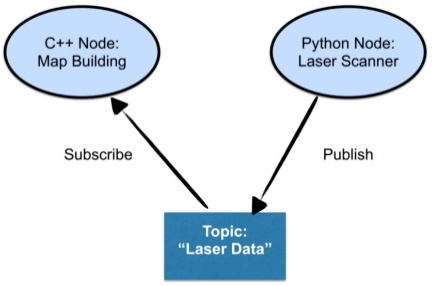
\includegraphics[width=0.5\linewidth]{Main/Chapter3/Images3/multilenguaje_1.png}
                \caption{Ejemplo de multilenguaje de ROS}
                \label{f:Cap3-5_multilenguaje_ros}
            \end{figure}

\newpage
            
        \subsubsection{Pequeño}
        
            Las convenciones ROS alientan a los contribuyentes a crear bibliotecas independientes y luego empaquetar esas bibliotecas para que puedan enviar y recibir mensajes hacia y desde otros módulos ROS. Esta capa adicional está destinada a permitir la reutilización de software fuera de ROS para otras aplicaciones, y simplifica en gran medida la creación de pruebas automatizadas utilizando herramientas de integración continua estándar.
            
        \subsubsection{Libre y Open Source}
        
            El núcleo de ROS se publica bajo la licencia BSD permisiva, que permite el uso comercial y no comercial. ROS pas\subsua datos entre módulos mediante comunicación entre procesos (IPC), lo que significa que los sistemas construidos con ROS pueden tener licencias detalladas de sus diversos componentes. Los sistemas comerciales, por ejemplo, a menudo tienen varios módulos de fuente cerrada que se comunican con una gran cantidad de módulos de fuente abierta. Los proyectos académicos y de pasatiempos suelen ser de código abierto. El desarrollo de productos comerciales a menudo se realiza completamente detrás de un firewall. Todos estos casos de uso, y más, son comunes y perfectamente válidos bajo la licencia ROS.
            
            \begin{figure}[htb]
                \centering
                
\includegraphics[width=0.3\linewidth]{Main/Chapter3/Images3/3-5/licnecia-bsd-ros.png}
                \caption{Licencia de ROS}
                \label{f:Cap3-5_multilenguaje_ros}
            \end{figure}
            

\newpage

    \subsection{Estadisticas}
    
    \subsubsection{Science Robotics}
        Science Robotics publico el articulo el 2017 “Powering the world’s robots 10 years of ROS” \cite{Zhangeaar1868} que habla sobre la iniciativa ROS-I (Ros Industrial) que se lanzó en 2012. Debido a las arquitecturas de software limitadas de los robots industriales actuales, es demasiado caro aplicar capacidades robóticas avanzadas para mejorar la productividad industrial. ROS-I proporciona interfaces para robots industriales comunes y dispositivos sensoriales junto con bibliotecas de software específicas para la automatización de la fabricación. ROS-I ha apoyado un número creciente de hardware industrial, como los robots producidos por ABB, Fanuc y Yaskawa. Además, el Consorcio ROS-I existe para desarrollar la comunidad ROS-I proporcionando apoyo técnico, organizando cursos de capacitación y talleres, y estableciendo la hoja de ruta para ROS-I. El Consorcio ROS-I tiene más de 50 miembros en todo el mundo, incluidos institutos de investigación y agencias gubernamentales, integradores de sistemas y usuarios finales, y fabricantes de equipos originales. Además, la próxima versión de ROS 2.0 debería abordar una de las principales limitaciones que ha ralentizado la adopción de ROS en la industria: que es una implementación de middleware interna. ROS 2.0 ahora se basa en el servicio de distribución de datos para la comunicación entre procesos, lo que brinda una confiabilidad mucho mejor con protocolos de calidad de servicio y seguridad con cifrado.

        La figura \ref{f:Cap3-5_estadisticas_1} muestra algunas estadísticas clave de ROS, las cuales son:

            \begin{figure}[htb]
                \centering
                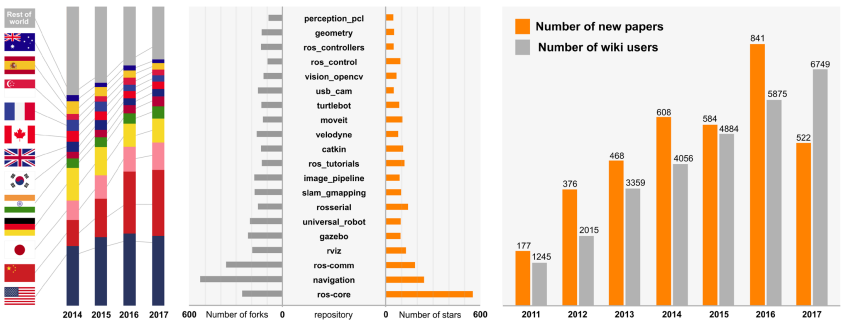
\includegraphics[width=1.0\linewidth]{Main/Chapter3/Images3/science_robot_esta_1.png}
                \caption{Estadísticas mundiales de ROS \cite{Zhangeaar1868}}
                \label{f:Cap3-5_estadisticas_1}
            \end{figure}        

        \begin{itemize}
            \item {Los países visitantes de la wiki de ROS en los últimos 4 años, muestra un cambio creciente de investigadores de países del Lejano Oriente (información recolectada del informe métrico anual de ROS). }
            \item {Los 20 principales repositorios ROS según la cantidad de bifurcaciones y estrellas (de Github, 10 de octubre de 2017).}
            \item {Artículos recientemente publicados en los últimos 10 años que han citado el artículo ''ROS original'' (de la búsqueda de Google Scholar, palabras clave “Sistema operativo de robot ROS”) y el número de usuarios de wiki registrados.}
        \end{itemize}
        

        La figura \ref{f:Cap3-5_estadisticas_2} muestra los diez años de desarrollos de ROS que respaldan la investigación y el desarrollo, incluida la robótica móvil, industrial, quirúrgica y espacial, así como los automóviles autónomos. Se han lanzado 11 distribuciones de ROS en los últimos 10 años, y el gráfico de barras muestra el número de descargas binarias de ROS en cada año. El Consorcio ROS-I se lanzó en 2013 con el objetivo de transformar las capacidades de ROS en tiempo real para robots industriales. ROS 2.0 es actualmente en desarrollo intenso, y se acaba de lanzar una versión beta.

            \begin{figure}[htb]
                \centering
                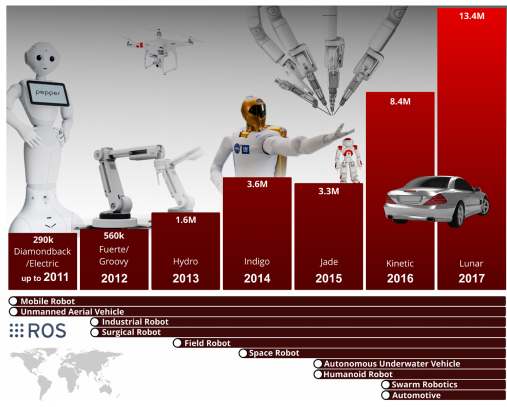
\includegraphics[width=1.0\linewidth]{Main/Chapter3/Images3/science_robot_esta_2.png}
                \caption{Desarrollo de ROS en los últimos 10 años \cite{Zhangeaar1868}}
                \label{f:Cap3-5_estadisticas_2}
            \end{figure}  


         \newpage
    
        \subsubsection{Metricas de la comunidad ROS}
    
    Ros Metrics miden aspectos de la comunidad ROS para comprender y rastrear el impacto de su trabajo e identificar áreas de mejora. Se inspiran en las métricas del Proyecto MeeGo .
    
        \begin{figure}[htb]
            \centering
            
\includegraphics[width=0.4\linewidth]{Main/Chapter3/Images3/cap3_estadisticas_3.png}
            \caption{Logo de ROS Metrics \cite{rosmetrics}}
            \label{f:Cap3-5_estadisticas_3}
        \end{figure}  
        
        Las figuras \ref{f:Cap3-5_estadisticas_4} y \ref{f:Cap3-5_estadisticas_5} presentan estadísticas recolectadas de la pagina oficial de ROS Metrics hasta el año 2021. Según la figura \ref{f:Cap3-5_estadisticas_4}, los países que más han visitado ROS son China, EEUU, Japón y Alemania. 
        
        \begin{figure}[htb]
            \centering
            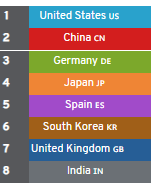
\includegraphics[width=0.27\linewidth]{Main/Chapter3/Images3/cap3_estadisticas_7.png}
            \caption{Top de países que utilizan ROS en base a la descarga de paquetes registrados hasta el 28 de marzo del año 2021 \cite{rosmetrics}.}
            \label{f:Cap3-5_estadisticas_4}
        \end{figure}  
        

        \begin{figure}[htb]
            \centering
            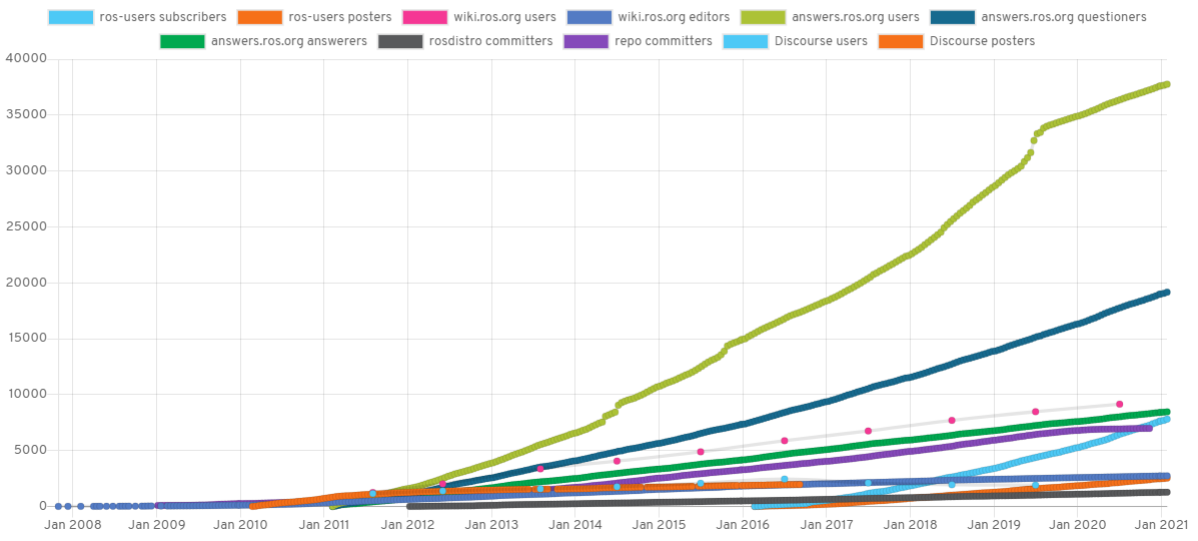
\includegraphics[width=1.0\linewidth]{Main/Chapter3/Images3/cap3_estadisticas_4.png}
            \caption{Colección de diferentes métricas para medir la cantidad de usuarios de la comunidad ROS \cite{rosmetrics}}
            \label{f:Cap3-5_estadisticas_5}
        \end{figure}  
        
        \newpage

        \subsubsection{Repositorio GitHub}
            Para comprender GitHub, primero se debe comprender Git. Git es un sistema de control de versiones de código abierto que fue iniciado por Linus Torvalds, la misma persona que creó Linux. Sirve para cuando los desarrolladores crean algo (una aplicación, por ejemplo), realizan cambios constantes en el código, lanzando nuevas versiones hasta y después del primer lanzamiento oficial. Los sistemas de control de versiones mantienen estas revisiones en orden, almacenando las modificaciones en un repositorio central. Esto permite a los desarrolladores colaborar fácilmente, ya que pueden descargar una nueva versión del software, realizar cambios y cargar la revisión más reciente. Todos los desarrolladores pueden ver estos nuevos cambios, descargarlos y contribuir. Del mismo modo, las personas que no tienen nada que ver con el desarrollo de un proyecto aún pueden descargar los archivos y usarlos. Git es una herramienta de línea de comandos, pero el centro alrededor del cual giran todas las cosas relacionadas con Git es el centro, GitHub.com, donde los desarrolladores almacenan sus proyectos y se conectan con personas de ideas afines.
    
            \begin{figure}[htb]
            \centering
            
\includegraphics[width=0.23\linewidth]{Main/Chapter3/Images3/repo_git_1.png}
            \caption{Logo GitHub, Inc.}
            \label{f:Cap3-5_estadisticas_8}
            \end{figure} 
        
            Dirk Thomas trabajo en ROS durante casi 9 años y envio 15 distribuciones de ROS. Uno del repositorio que subió a GitHub registra el total de autores, commits y repositorios en Github con relación a ROS hasta octubre del 2020.
        
            \begin{figure}[htb]
            \centering
            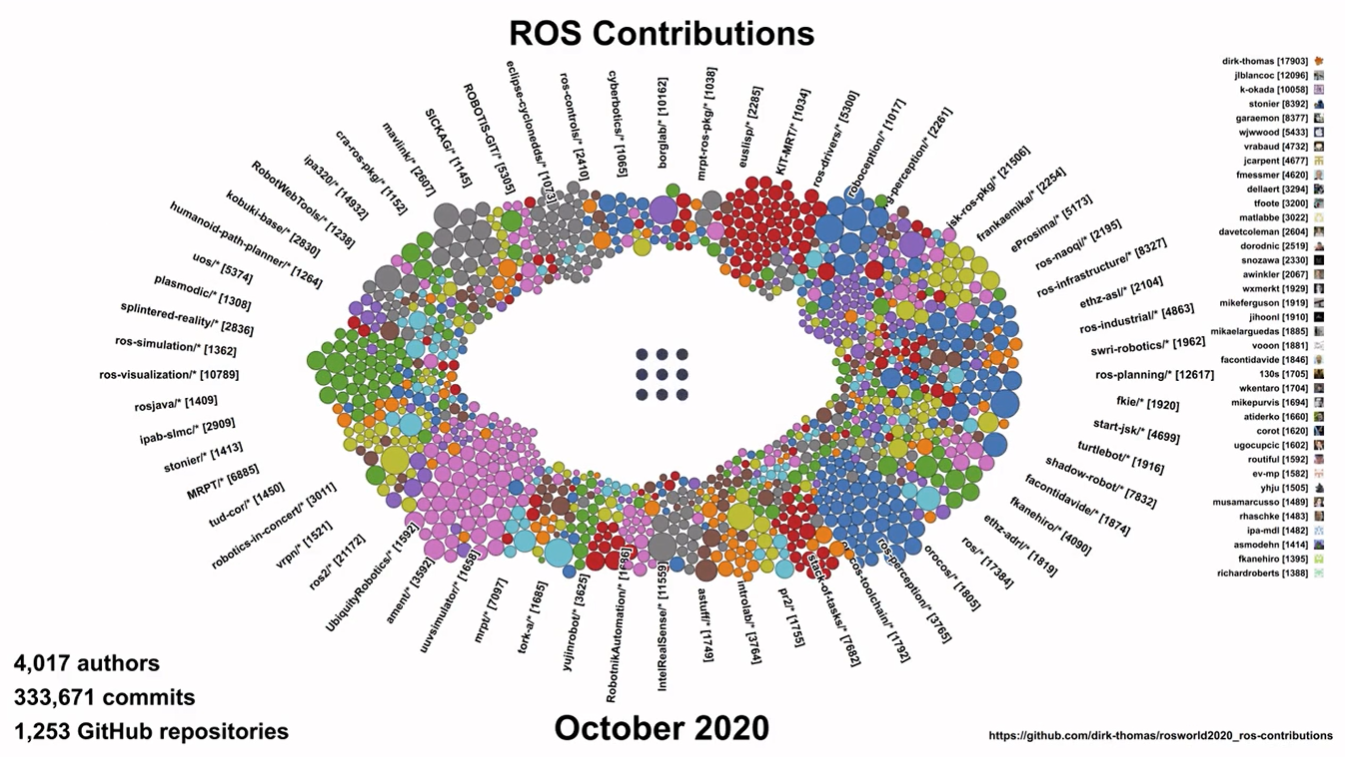
\includegraphics[width=0.99\linewidth]{Main/Chapter3/Images3/repo_git_2.png}
            \caption{Visualización de las contribuciones de ROS en GitHub \cite{gitreposito}}
            \label{f:Cap3-5_estadisticas_9}
            \end{figure} 
    
        \newpage

    \subsection{Versiones}
            En 2007, Willow Garage logró la investigación del marco de software de robot que comenzó en el laboratorio de inteligencia artificial de la Universidad de Stanford y continuó el desarrollo bajo el nombre de Robot Operating System. Con la sexta versión de lanzamiento oficial "ROS Groovy Galápagos", Willow Garage intentó penetrar en el mercado de robots de servicios comerciales en 2013, pero terminó dividiéndose en varias empresas emergentes y finalmente se entregó a la Open Source Robotics Foundation. Desde entonces, se lanzaron 4 versiones más y, a partir de mayo de 2017, OSRF cambió su nombre a Open Robotics y ha estado desarrollando, operando y administrando ROS. Más recientemente, la undécima versión de ROS, ROS Lunar Loggerhead, fue lanzada el 23 de mayo de 2017. ROS etiqueta la primera letra de cada nombre de lanzamiento en orden alfabético y usa una tortuga como su símbolo (ver figura \ref{f:Cap3-5_estadisticas_10}).
            
            \begin{figure}[htb]
            \centering
            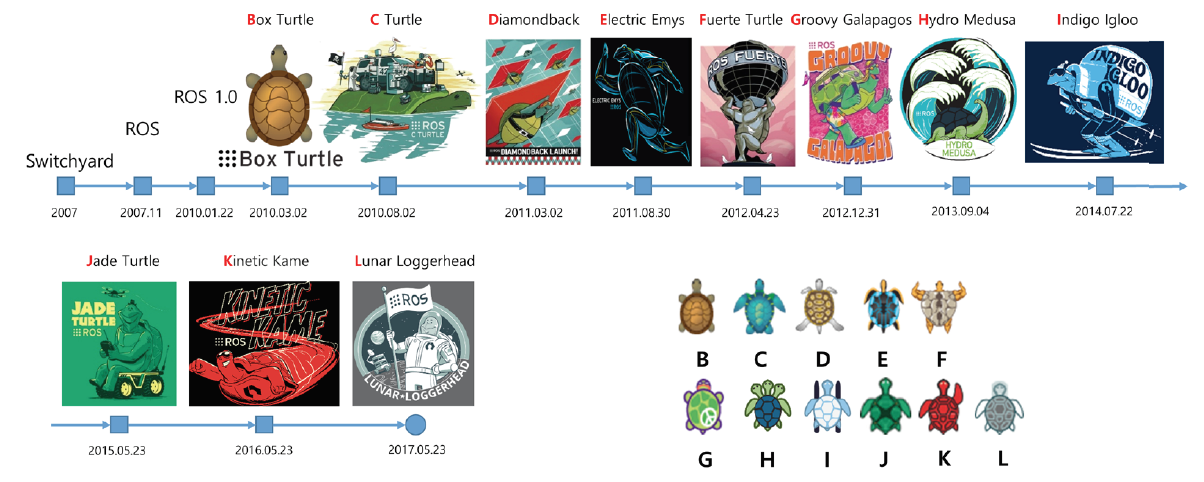
\includegraphics[width=0.94\linewidth]{Main/Chapter3/Images3/ver_ros_1.png}
            \caption{Linea temporal e iconos de tortuga para cada versión de ROS \cite{ROS_BOOK_1}}
            \label{f:Cap3-5_estadisticas_10}
            \end{figure} 
    
            \begin{figure}[htb]
            \centering
            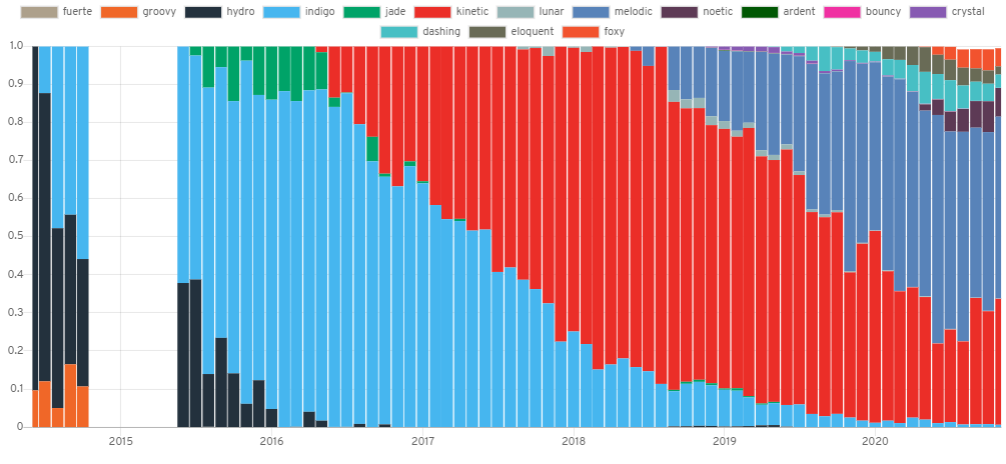
\includegraphics[width=0.94\linewidth]{Main/Chapter3/Images3/ver_ros_2.png}
            \caption{Uso relativo de cada versión de ROS basado en descargas de packages.ros.org \cite{rosmetrics}.}            \label{f:Cap3-5_estadisticas_11}
            \end{figure} 
    
    \newpage
    
    \subsection{Conceptos principales}
            
            Hay tres niveles de conceptos en ROS. El primero se refiere a cómo diferentes archivos están organizados en la computadora, herramientas ROS para administrar código fuente, instrucciones de compilación y definiciones de mensajes (nivel de sistema de archivos). El segundo son los componentes de la red peer to peer de nodos ROS, es decir, los procesos. (nivel de gráfico computacional). Por último, el nivel 3 es en relación a cómo los usuarios comparten software para permitir que todos lo utilicen (nivel comunitario).
            
            \begin{figure}[htb]
                \centering
                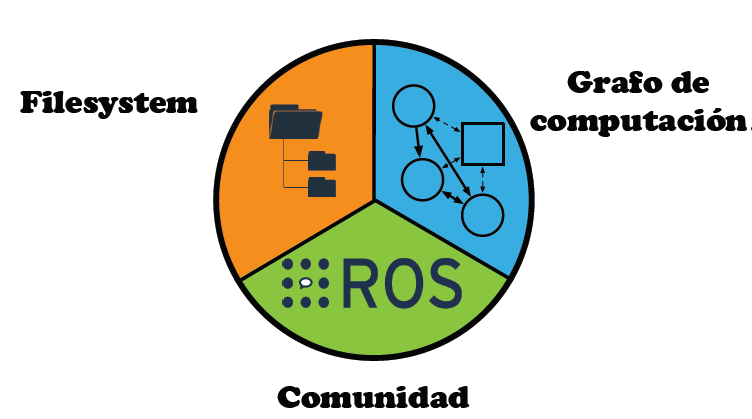
\includegraphics[width=1\linewidth]{Main/Chapter3/Images3/nivel_s_a_1.png}
                \caption{Niveles de conceptos de ROS}
                \label{f:Cap3_conceptos_1}
            \end{figure} 
            

                
                
               \newpage
               
            \subsubsection{Nivel de sistemas de archivos}

                Similar a un sistema operativo, los archivos de ROS también se organizan en el disco duro de una manera particular. En este nivel, se puede ver cómo se organizan estos archivos en el disco. La figura \ref{f:Cap3_conceptos_2} muestra cómo se organizan los archivos y carpetas:
                
                
            \begin{figure}[htb]
                \centering
                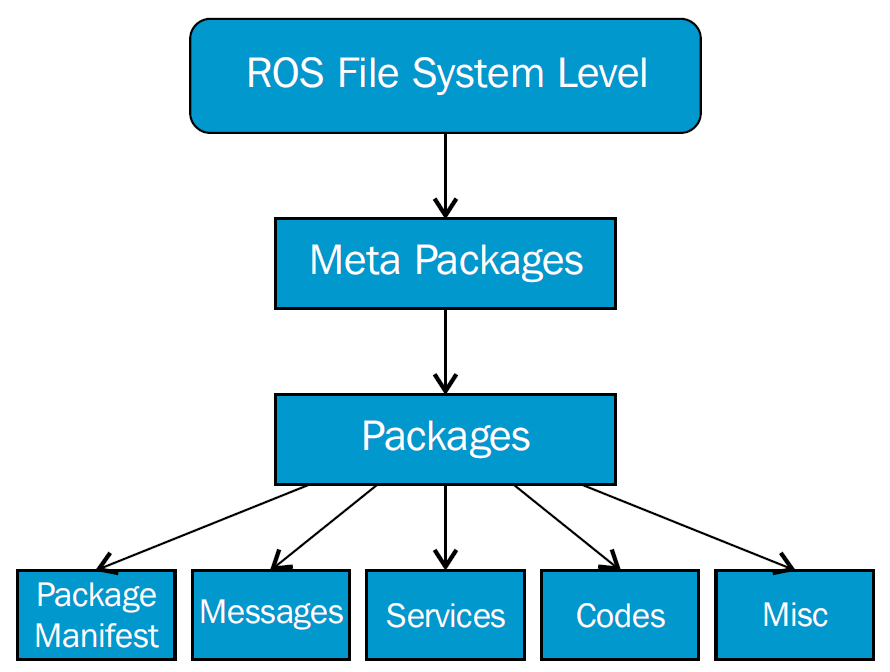
\includegraphics[width=0.55\linewidth]{Main/Chapter3/Images3/n_s_a_2.png}
                \caption{Nivel de sistema de archivos ROS \cite{lentin_2015}}
                \label{f:Cap3_conceptos_2}
            \end{figure} 
                
                

            A cuntinuacion se presenta la descripcion de cada bloque en el sistema de archivos:
            \begin{itemize}
                \item {\textbf{Meta packages:} Es un único paquete lógico compuesto por muchos paquetes en su interior. Además, los meta paquetes contienen un archivo package.xml que describe la carpeta y sus dependencias.}
                \item {\textbf{Packages:} Son las unidades más bajas y la principal para organizar el software en ROS. Un paquete puede contener procesos en tiempo de ejecución ROS (nodos), un Biblioteca dependiente de ROS, conjuntos de datos, archivos de configuración o achivos de lanzamiento. Cada directorio de paquete debe incluir un archivo CMakeList.txt y package.xml que describa el contenido del paquete y cómo catkin debe interactuar con él.}
                \item {\textbf{Stacks:} Son grupos de paquetes que se juntan para realizar funciones de alto nivel.}
                \item {\textbf{Manifests:} Los manifiestos proporcionan metadatos sobre un paquete. Pueden pertenecer a un packages o una Stacks y describen información general sobre un paquete o Stacks específico, como una breve descripción de lo que hace, el nombre del autor, su tipo de licencia y las dependencias.con otros paquetes.}
                \item {\textbf{Message (msg) types:} Las descripciones de los mensajes definen los datos estructuras para mensajes enviados en ROS.}
                \item {\textbf{Service (srv) types:} Las descripciones de servicio definen la solicitud y estructuras de datos de respuesta para servicios en ROS.}
            \end{itemize}
            
               \newpage
               
            ROS está basado en CMake y puede ser utilizado por muchos sistemas operativos como Linux o Windows. CMake es un generador de herramientas de creación, una herramienta de nivel superior, que simplifica el proceso de compilación y construcción, puede gestionar grandes proyectos y tiene una buena escalabilidad. Para una plataforma a gran escala como ROS, se usa CMake, y ROS ha extendido CMake, por lo que hay un sistema de compilación Catkin. Catkin es el sistema de compilación de ROS que genera programas ejecutables, bibliotecas e interfaces y proporciona el concepto de espacio de trabajo en la construcción de cada proyecto.
            
            La estructura del espacio de trabajo catkin, incluye las carpetas src, build, devel. Las tres rutas también pueden incluir otras en algunas opciones de compilación. Pero estas tres carpetas son las predeterminadas para el sistema de compilación catkin. Sus roles específicos son los siguientes:

            \begin{itemize}
                \item {\textbf{Espacio fuente (src):} Contiene el código fuente donde el usuario puede extraer, verificar o clonar el código fuente de los paquetes que quiere construir.}
                \item {\textbf{Espacio de construcción (build):} Este es el espacio donde CMake apela para construir los paquetes en el espacio de trabajo de catkin. CMake y Catkin mantienen su información de caché y otros intermedios archivos.}
                \item {\textbf{Espacio de desarrollo (devel):} Se encuentran archivos de objetos generados (incluidos archivos de encabezado, bibliotecas de vínculos dinámicos, bibliotecas de vínculos estáticos, archivos ejecutables, etc.), variables de entorno}
            \end{itemize}


            Durante el proceso de compilación, el flujo de trabajo de un catkin workspace es el que se muestra con flechas azules en la figura \ref{f:Cap3_conceptos_3}. Los dos últimos procesos son generados y administrados automáticamente por el sistema catkin. El uso principal para los usuarios de ROS es la carpeta src\/, donde los paquetes creados o copiados se almacenan en dicha carpeta. En el momento de la compilación, el sistema de compilación de catkin busca y compila todos los paquetes de código fuente de forma de src\/.

            \begin{figure}[htb]
                \centering
                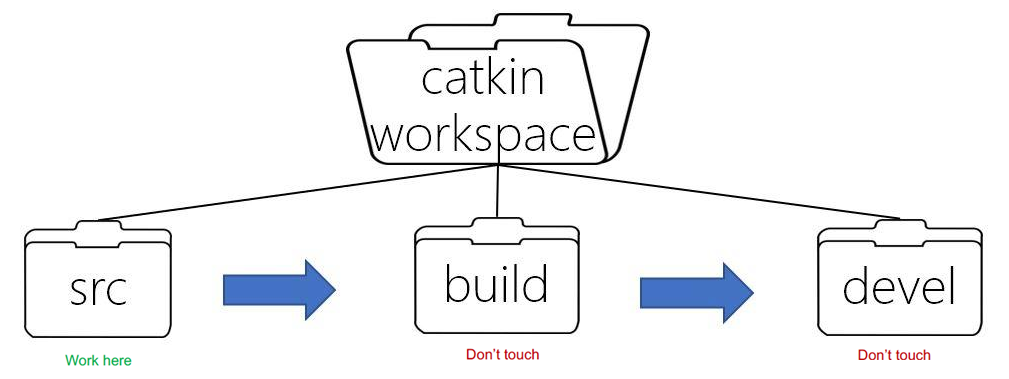
\includegraphics[width=0.8\linewidth]{Main/Chapter3/Images3/n_s_a_3.png}
                \caption{Espacio de trabajo catkin\_make \cite{cmake_blogcsdn}}
                \label{f:Cap3_conceptos_3}
            \end{figure} 
            
               \newpage


            Cuando se crea un paquete, normalmente es común encontrar las carpetas de la figura \ref{f:Cap3_conceptos_4} dentro de el:
            
            \begin{figure}[htb]
                \centering
                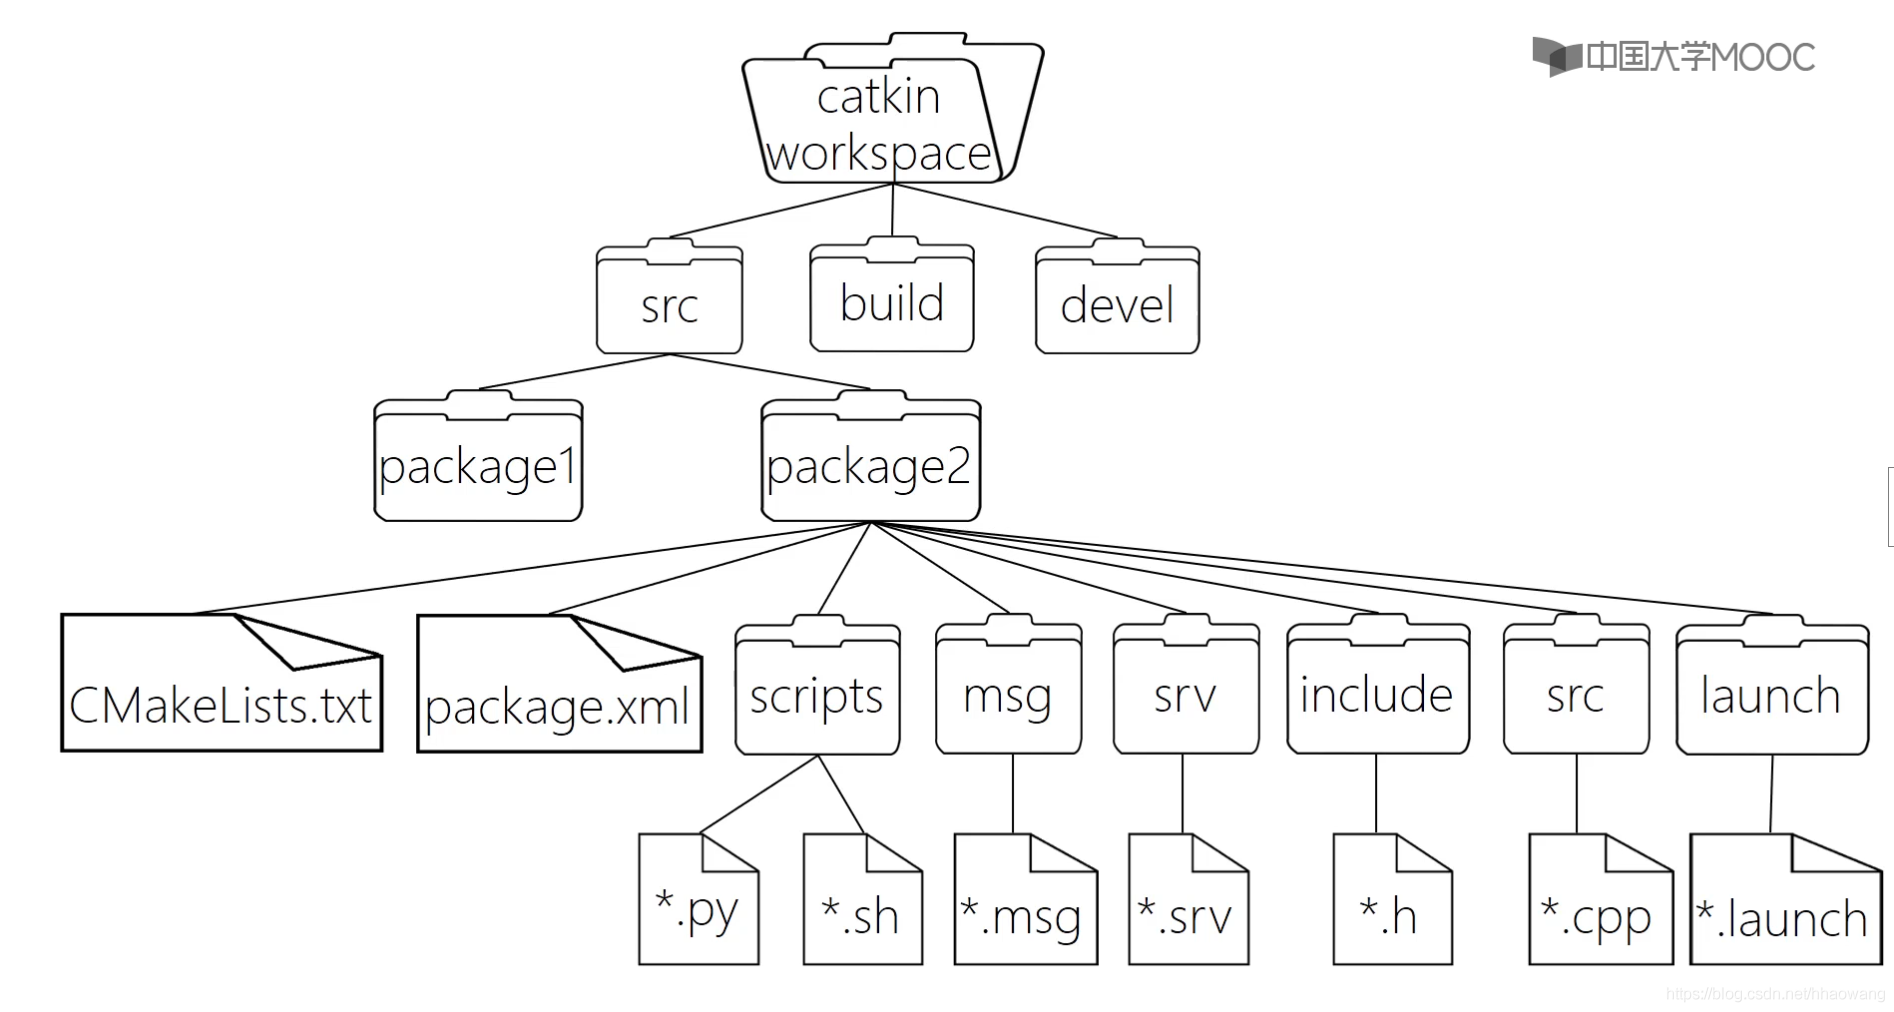
\includegraphics[width=1.0\linewidth]{Main/Chapter3/Images3/n_s_a_4.png}
                \caption{Estructura y características de catkin\_make \cite{cmake_blogcsdn}}
                \label{f:Cap3_conceptos_4}
            \end{figure} 

            \begin{itemize}
                \item {\textbf{/include/:} Esta carpeta contiene los encabezados (*.h) y las bibliotecas (*.lib, *.so).}
                \item {\textbf{/config/:} Todas las configuraciones se almacenan en esta carpeta incluidos los parámetros definidos, como controlador de robot con una extensión (*.yaml).}
                \item {\textbf{/launch/:} Contiene los archivos (*.launch) para ejecutar los nodos seleccionados del paquete o de otros paquetes usando el comando <incluir/>.}
                \item {\textbf{/msg/:} Contiene el tipo de datos del mensaje para nuestra aplicación (*.msg).}
                \item {\textbf{/srv/:} Esta carpeta contiene el tipo de mensaje para los servicios (*.srv).}
                \item {\textbf{/actions/:} Contiene el tipo de datos del mensaje utilizado en las acciones (*.action). }
                \item {\textbf{/src/:} Todo el código que se va a computar en el paquete debe estar dentro de esta carpeta con extensión (*.cpp).}
                \item {\textbf{package.xml:} Descripción del paquete y lista de dependencias utilizadas por el.}
                \item {\textbf{CmakeLists.txt:} Lista de requisitos y dependencias que debe compilar el ejecutador del paquete.}
            \end{itemize}

\newpage
            \subsubsection{Nivel gráfico computacional}
            
            El nivel gráfico computacional describe la infraestructura que utilizan los componentes ROS para comunicarse. Se basa en una red de procesos peer-to-peer (nodos) y se compone de varias unidades tales como las de la figura \ref{f:Cap3_conceptos_5}:
            
            \begin{figure}[htb]
                \centering
                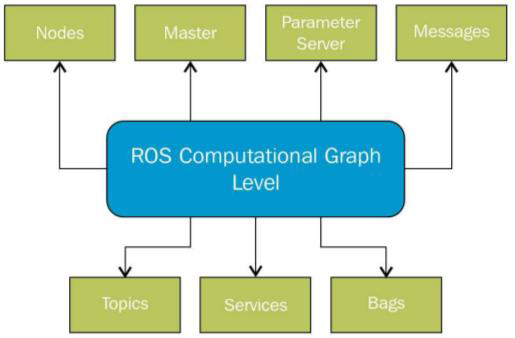
\includegraphics[width=0.63\linewidth]{Main/Chapter3/Images3/n_s_a_5.png}
                \caption{Estructura de la capa ROS Graph \cite{lentin_2015}}
                \label{f:Cap3_conceptos_5}
            \end{figure} 
            
            \paragraph{Nodes (Nodos)}
                   Son ejecutables en el sistema ROS y realizan la parte computacional. Se pueden conectar a otros nodos mediante 2 tipos de comunicación: Publisher/Subscriber o Services. Cada nodo tiene su propio nombre para ser reconocido y distinguido de los demás nodos. En ROS existen muchos lenguajes para programar un nodo como C ++, Python o Java. 
                   
            \paragraph{Ros Master}
                    Ros Master habilita el funcionamiento de la red ROS y es el primer proceso que debe ejecutarse cuando estamos usando ROS. Su función es registrar todos los nodos que se ejecutan y los temas y servicios existentes. Esto es esencial para interconectar nodos y monitorear todas las unidades en el sistema
            \begin{figure}[htb]
                \centering
                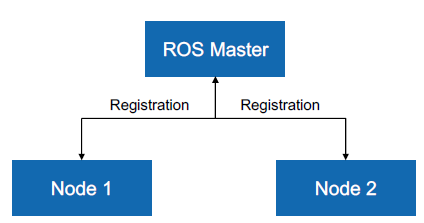
\includegraphics[width=0.55\linewidth]{Main/Chapter3/Images3/n_s_a_6.png}
                \caption{Registro de nodos en ROS Master \cite{rosmaster_diagram}.}
                \label{f:Cap3_conceptos_6}
            \end{figure} 
            
            
               \newpage


            \paragraph{Topics (Temas)}
                Los nodos comparten información pasando y recibiendo mensajes. Estos mensajes se publican con un nombre especial llamado tema. Por lo tanto, los nodos pueden publicar o suscribirse a un tema específico para obtener los mensajes deseados. Muchos nodos se pueden suscribir al mismo tema para recibir los mensajes que necesitan. Las comunicaciones entre nodos se realizan de forma unidireccional, por lo que cualquier nodo que envíe la información sobre un tema no puede recibir respuesta en el mismo canal, ni saber si el nodo receptor ha recibido el mensaje.
            \begin{figure}[htb]
                \centering
                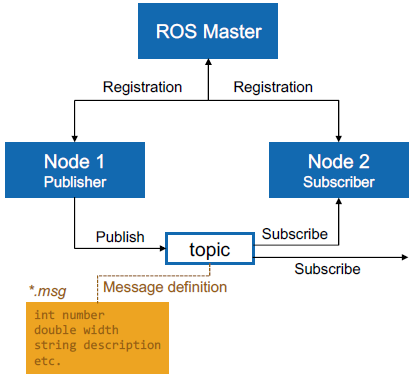
\includegraphics[width=0.68\linewidth]{Main/Chapter3/Images3/n_s_a_7.png}
                \caption{Nodos comunicándose a través de topic por medio de un mensaje *.msg \cite{rosmaster_diagram}.}
                \label{f:Cap3_conceptos_7}
            \end{figure} 
            \begin{figure}[htb]
                \centering
                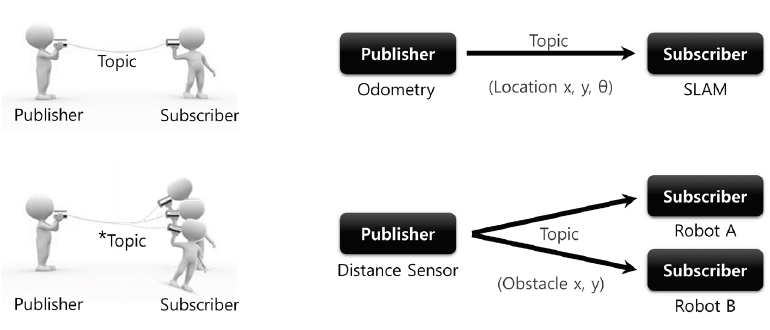
\includegraphics[width=0.92\linewidth]{Main/Chapter3/Images3/n_s_a_8.PNG}
                \caption{Comunicación de mensajes por medio de topics \cite{ROS_BOOK_1}}
                \label{f:Cap3_conceptos_8}
            \end{figure} 


               \newpage


            \paragraph{Services (Servicios)}
                 Aunque el principal método de comunicación entre nodos es a través de temas, ya que explicado anteriormente, existe otra metodología en ROS llamada llamadas de servicio. Las llamadas de servicio ROS son diferentes de mensajes debido a las siguientes características: son bidireccionales y uno a uno. 
                 
                Este proceso síncrono de comunicación se basa en un sistema cliente / servidor o solicitud / respuesta., donde un nodo cliente envía algunos datos llamados solicitud a un nodo servidor y espera hasta que el servidor pueda responder. Los servidor, habiendo recibido esta solicitud, toma alguna acción  y enviar algunos datos llamados respuesta al nodo cliente
                La descripción del servicio se almacena en un archivo de definición de servicio *.msg, guardado en un subdirectorio /srv. 

            \begin{figure}[htb]
                \centering
                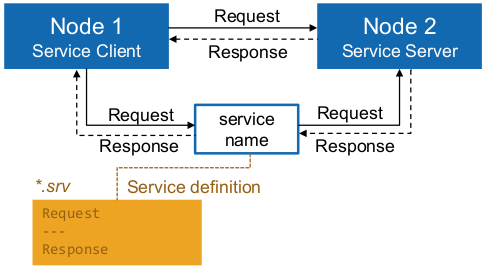
\includegraphics[width=0.85\linewidth]{Main/Chapter3/Images3/n_s_a_9.png}
                \caption{Comunicación request/response entre nodos que realizan servicios \cite{rosmaster_diagram}.}
                \label{f:Cap3_conceptos_9}
            \end{figure} 
            
            \begin{figure}[htb]
                \centering
                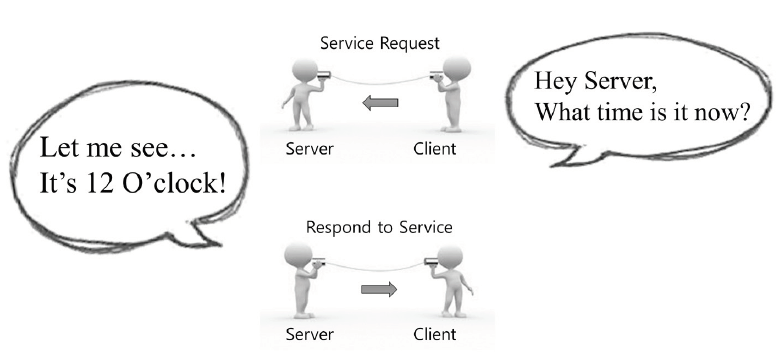
\includegraphics[width=1.0\linewidth]{Main/Chapter3/Images3/n_s_a_10.PNG}
                \caption{Comunicación de mensajes de servicio \cite{ROS_BOOK_1}.}
                \label{f:Cap3_conceptos_10}
            \end{figure}             

               \newpage

            \paragraph{ Actions (Acciones)}
                    Una acción es una comunicación bidireccional asíncrona entre los nodos activos basados en el cliente de la acción y el sistema del servidor de la acción que se muestra en la figura \ref{f:Cap3_conceptos_11}. El sistema de acción, como los servicios explicados anteriormente, envía algo del cliente de acción de datos al servidor de acción llamado objetivo y el servidor de acción responde un resultado. Las acciones se diferencian de los servicios porque el servidor puede proporcionar retroalimentación y estado al cliente en cualquier momento sobre el proceso que se está realizando y el nodo cliente puede cancelar el objetivo anterior requerido para el servidor en cualquier momento también.
                    Al igual que en las llamadas de servicio ROS, las acciones deben definir pocos mensajes para comunicar al cliente con el servidor. Esto es posible gracias a las especificaciones de acciones, que definen estos mensajes en un archivo de acción con extensión *.action. Estos archivos generalmente se almacenan en una subcarpeta /action/ en el directorio del paquete.
                    El archivo * .action se divide en 3 secciones. Cada parte está separada por 3 guiones (---). En la primera parte se define el objetivo, en la segunda se establece la retroalimentación y en la última se especifica la definición del resultado.

            \begin{figure}[htb]
                \centering
                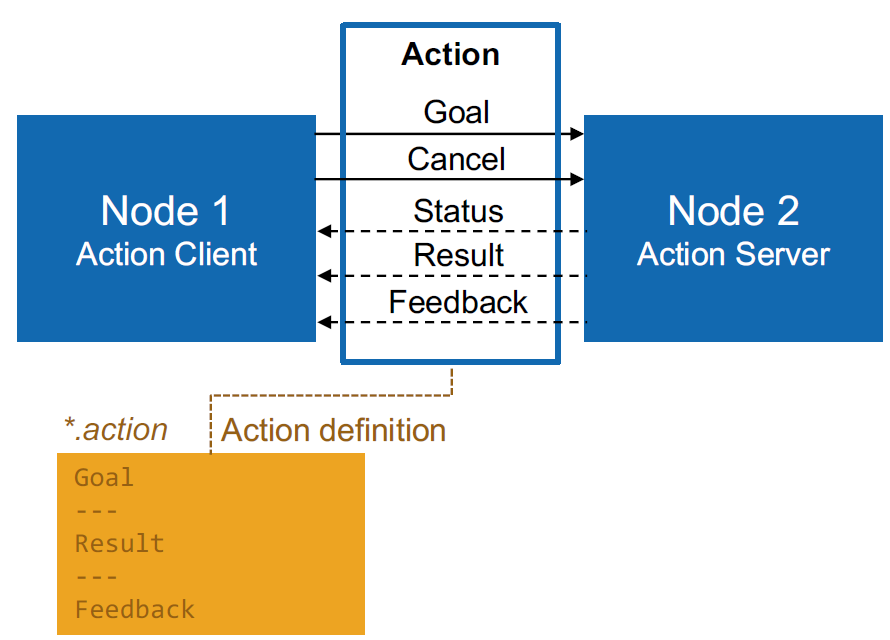
\includegraphics[width=0.7\linewidth]{Main/Chapter3/Images3/action_diagram.png}
                \caption{Comunicación bidireccional entre nodos por medio de acciones \cite{rosmaster_diagram}.}
                \label{f:Cap3_conceptos_11}
            \end{figure}             

            \begin{figure}[htb]
                \centering
                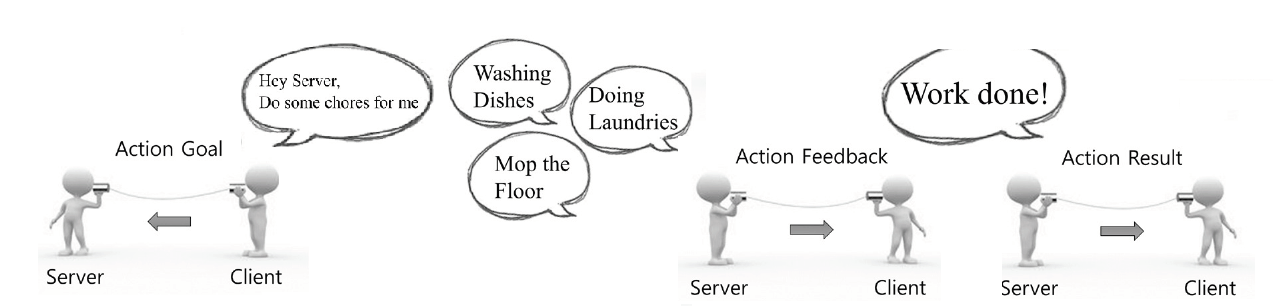
\includegraphics[width=1.0\linewidth]{Main/Chapter3/Images3/n_s_a_12.png}
                \caption{Comunicación de mensajes de acción \cite{ROS_BOOK_1}.}
                \label{f:Cap3_conceptos_12}
            \end{figure}   

               \newpage

            \paragraph{Messages (Mensajes)}
                Un mensaje es simplemente una estructura de datos, que comprende campos escritos. Tipos primitivos estándar (entero, punto flotante, booleano, etc.) son compatibles (figura \ref{f:Cap3_conceptos_13}). En muchos paquetes utilizados en ROS se incluyen mensajes especiales llamados 'encabezado', que son básicamente mensajes creados por otros. Hay tres campos definidos en un mensaje de encabezado: 
                
                \begin{itemize}
                    \item {\textbf{uint32 seq:} Corresponde al número del mensaje enviado por un editor determinado}
                    \item {\textbf{time stamp: } La hora exacta a la que se envió el mensaje}
                    \item {\textbf{string frame\_id:} Muestra el sistema de referencia utilizado}
                \end{itemize}

            \begin{figure}[htb]
                \centering
                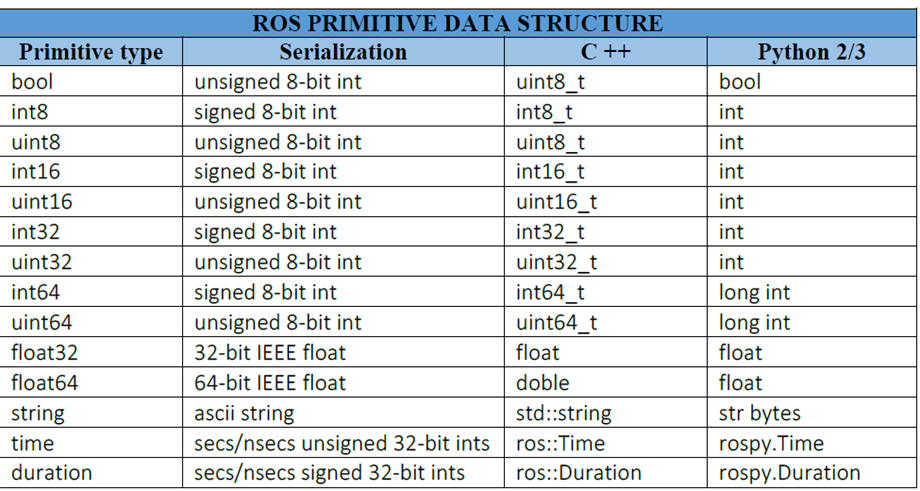
\includegraphics[width=1.0\linewidth]{Main/Chapter3/Images3/n_s_a_13.png}
                \caption{Tipos de datos basicos para mensajes en ROS \cite{ROS_BOOK_1}.}
                \label{f:Cap3_conceptos_13}
            \end{figure}   

            \paragraph{ Parameter Server (Servidor de parámetros)}
                 El servidor de parámetros permite que los datos se almacenen por clave en una ubicación. Actualmente forma parte del Máster.Básicamente es un almacén de constantes.

               
            \paragraph{Bags (Bolsas)}
            Las bolsas son un formato para guardar y reproducir datos de mensajes ROS. Las bolsas son un mecanismo importante para almacenar datos, como los datos de los sensores, que pueden ser difíciles de recopilar, pero son necesarios para desarrollar y probar algoritmos
               \newpage
               
            \paragraph{Esquema resumen de nivel gráfico}
                El sistema ROS permite que diferentes nodos se comuniquen entre sí, intercambiando información y datos. Sin embargo, todo el sistema necesita un ROS Master en ejecución para notar la existencia de otros nodos y comenzar a comunicarse entre sí. El ROS Master permite que los nodos ROS individuales se ubiquen entre sí en el sistema y rastrea a los editores y suscriptores a temas y servicios. Un nodo es generalmente un pequeño programa escrito en Python o C ++ que ejecuta alguna tarea o proceso relativamente simple. Los nodos se pueden iniciar y detener de forma independiente entre sí y se comunican pasando mensajes. Un nodo puede publicar mensajes sobre determinados temas, proporcionar servicios o acciones entre otros nodos. 
                
                
                
            \begin{figure}[htb]
                \centering
                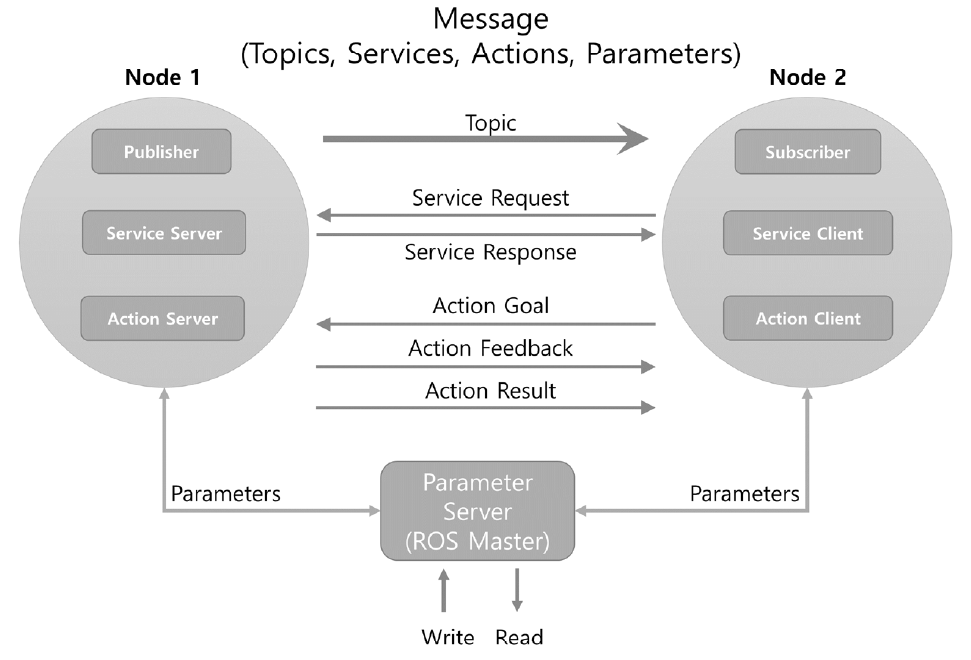
\includegraphics[width=1.0\linewidth]{Main/Chapter3/Images3/n_s_a_14.PNG}
                \caption{Comunicación de mensajes entre nodos \cite{ROS_BOOK_1}}
                \label{f:Cap3_conceptos_14}
            \end{figure}   

               \newpage
               
            \subsubsection{Nivel Comunitario}
            
            El ecosistema ROS ahora consta de decenas de miles de usuarios en todo el mundo, que trabajan en dominios que van desde proyectos de pasatiempos de mesa hasta grandes sistemas de automatización industrial. 
            Una característica importante de ROS es la comunidad que comparte software y código, lo que convierte a ROS en una de las comunidades de robots más grandes. Hay diferentes formas de obtener recursos ROS:

            \begin{figure}[htb]
                \centering
                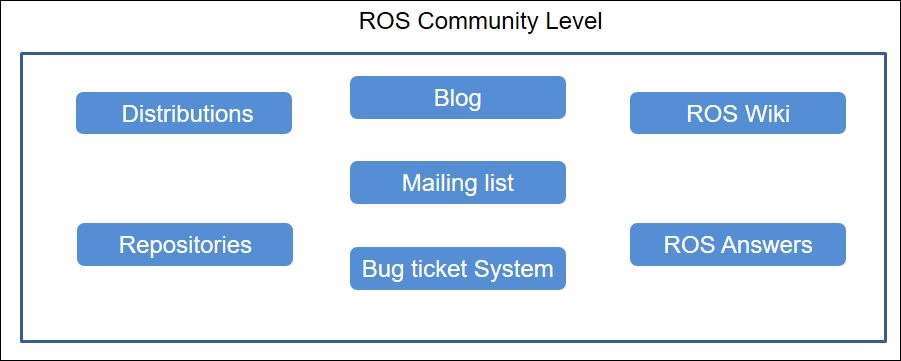
\includegraphics[width=0.9\linewidth]{Main/Chapter3/Images3/n_s_a_15.png}
                \caption{Nivel comunitario de ROS \cite{lentin_2017}}
                \label{f:Cap3_conceptos_15}
            \end{figure}        
            
            \begin{itemize}
                \item {\textbf{Distribuciones:} las distribuciones ROS son colecciones de stacks versionadas que puede instalar. Las distribuciones juegan un papel similar a las distribuciones de Linux: facilitan la instalación de una colección de software y también mantienen versiones consistentes en un conjunto de software. (http://wiki.ros.org/Distributions)}
                \item {\textbf{Repositorios:} ROS se basa en una red federada de repositorios de código, donde diferentes instituciones pueden desarrollar y lanzar sus propios componentes de software de robot. }
                \item {\textbf{El ROS Wiki:} La Wiki de la comunidad de ROS es el foro principal para documentar información sobre ROS. Cualquiera puede registrarse para obtener una cuenta y contribuir con su propia documentación, proporcionar correcciones o actualizaciones, escribir tutoriales y más. (http://wiki.ros.org/) }
                \item {\textbf{Mailing Lists:} Listas de correo de usuarios ROS}
                \item {\textbf{Answers:} Página web donde los usuarios comparten preguntas, respuestas y comentarios. (https://answers.ros.org/) }
                \item {\textbf{Blog ROS:} Noticias de la comunidad ROS. (www.ros.org/news/)  }
                \item {\textbf{ROS Discourse:} es el foro de discusión de la comunidad (https://discourse.ros.org/). No es para cuestiones técnicas específicas, sino para temas, anuncios y noticias más amplio.}
            \end{itemize}
            
            
            
            
               \newpage
               
    \newpage

    \subsection{Herramientas}
    
        Existen varias herramientas que pueden ayudarnos a la hora de usar ROS. Debemos tener en cuenta estas herramientas GUI como complementarias a las herramientas de línea de comandos. Hay una gran cantidad de herramientas ROS, incluidas las herramientas que los usuarios de ROS también han lanzado personalmente. Entre estas herramientas, las que discutiremos en este capítulo no procesan directamente una función en el ROS, pero son herramientas complementarias muy útiles para programar con ROS.
            
        \subsubsection{Launch Files}
            En un proyecto ROS, es posible que desee ejecutar varios nodos ROS al mismo tiempo para realizar sistemas más complejos. ROS tiene una herramienta llamada roslaunch que permite a los usuarios ejecutar numerosos nodos, establecer parámetros de configuración de cada nodo, renombrar los nombres de temas predeterminados e incluso cambiar el nombre del nodo. El propósito de esto es configurar fácilmente el sistema global.
            
        \subsubsection{RQT Graph}
            Proporciona visualización de un sistema ROS, mostrando los nodos y las conexiones entre ellos que permite depurar y comprender el sistema en ejecución y cómo está estructurado. 
            
            \begin{figure}[htb]
                \centering
                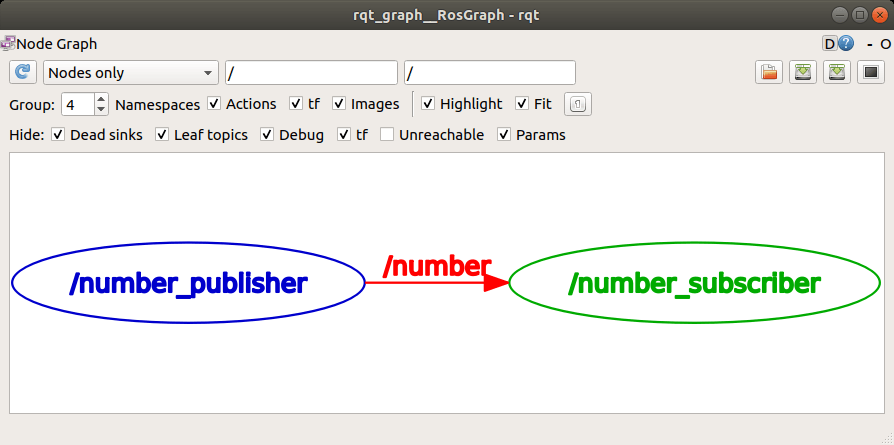
\includegraphics[width=1.0\linewidth]{Main/Chapter3/Images3/herramientas_1.png}
                \caption{Visualización de la comunicación entre un nodo publisher y el nodo subscriber a travez del tema number en RQT Graph.

}
                \label{f:Cap3_herramientas_1}
            \end{figure}       
            
            
    \newpage    
    
            \subsubsection{RQT Rosbag}
                Rosbag es un conjunto de herramientas para grabar y reproducir datos de temas ROS. Los datos se almacenan en archivos de bag y hay disponibles herramientas de línea de comandos para trabajar con bag. Rosbag evita la deserialización y reserialización de mensajes y sus principales herramientas son:
                
                    \begin{itemize}
                        \item{\textbf{rosbag info:} Muestra el contenido de los archivos de la bolsa, como temas grabados, hora de inicio y finalización, número de mensajes, frecuencia y estadísticas de compresión} 
                        \item{\textbf{rosbag record:} Escribe el contenido de todos los mensajes publicados sobre esos temas que queremos registrar y la información se almacena en un archivo .bag.} 
                        \item{\textbf{rosbag play: } Lee un archivo de bolsa y publica la información sobre temas ROS de forma sincronizada en el tiempo. El sistema ROS puede utilizar esta información como si fuera en tiempo real.} 
                    \end{itemize}

            \subsubsection{RQT reconfigure}
Adaptación del paquete “Dynamic reconfigure” que permite modificar en tiempo real todos los parámetros de los nodos, para realizar modificaciones rapidas. La configuración de los parámetros se puede exportar para utilizar en el futuro.

            \subsubsection{MoveIt }
 Software basado en la planificación del movimiento, que considera prospección 3D, cinemática, control y navegación. Proporciona una plataforma para el desarrollo de aplicaciones robóticas, evalúa nuevos diseños de robots y productos para la construcción robótica integrado para aplicaciones industriales, I + D, etc.
 
             \begin{figure}[htb]
                \centering
                
\includegraphics[width=0.8\linewidth]{Main/Chapter3/Images3/herramientas_2.png}
                \caption{Logo Proyecto MoveIt}
                \label{f:Cap3_herramientas_2}
            \end{figure}     
            
        \newpage    

            \subsubsection{Gazebo}
     Es un simulador virtual que brinda la posibilidad de realizar simulaciones de algoritmos, diseños de robots y ejecutar pruebas dentro de escenarios reales con precisión y eficiencia. Proporciona un motor de física robusto, gráficos de alta calidad e interfaces gráficas. 
        
        \begin{figure}[htb]
                \centering
                
\includegraphics[width=0.3\linewidth]{Main/Chapter3/Images3/herramientas_4.png}
                \caption{Logo Gazebo}
                \label{f:Cap3_herramientas_4}
        \end{figure} 
    
        
        \begin{figure}[htb]
                \centering
                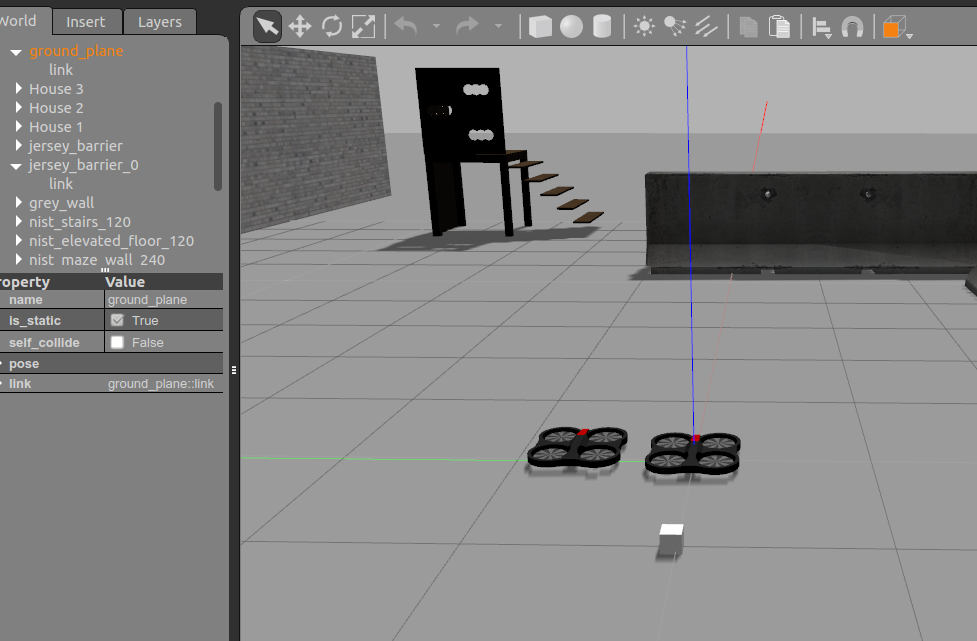
\includegraphics[width=0.98\linewidth]{Main/Chapter3/Images3/herramientas_3.png}
                \caption{Simulación de dron en Gazebo}
                \label{f:Cap3_herramientas_3}
        \end{figure}  

    
        \newpage    



\section{Visualización}
    
    \subsection{Interfaz de visualización gráfica ROS visualization (Rviz)}

        RVIZ es la abreviación de ROS visualización. Es un entorno de visualización 3D de uso general para robots, sensores y algoritmos. Permite visualizar mapas, robots, objetos, datos láser, imágenes de cámaras, nubes de puntos y marcadores.   Como la mayoría de las herramientas ROS, se puede utilizar para cualquier robot y configurar rápidamente para una aplicación en particular.
        
        \begin{figure}[htb]
            \centering
            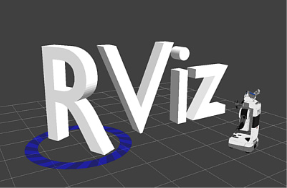
\includegraphics[width=0.35\linewidth]{Main/Chapter3/Images3/3-6/logo-rviz.png}
            \caption{Logo de Rviz}
            \label{f:Cap3-6_logo_rviz}
        \end{figure}
        
        RVIZ proporciona una interfaz sencilla para elegir la información que queremos que se muestre. La Figura 3.2 muestra un ejemplo de la interfaz RVIZ. A la izquierda podemos ver todos los elementos que muestra RVIZ. Cada elemento debe configurarse con el nombre de un tema específico. Entonces RVIZ se suscribe a ese tema y visualiza su información. En el medio está la ventana principal donde se muestra toda la información y a la izquierda podemos elegir las propiedades de la herramienta y cambiar entre diferentes vistas. RVIZ también permite al usuario crear complementos para agregar nuevas capacidades de visualización.
        
        \begin{figure}[htb]
            \centering
            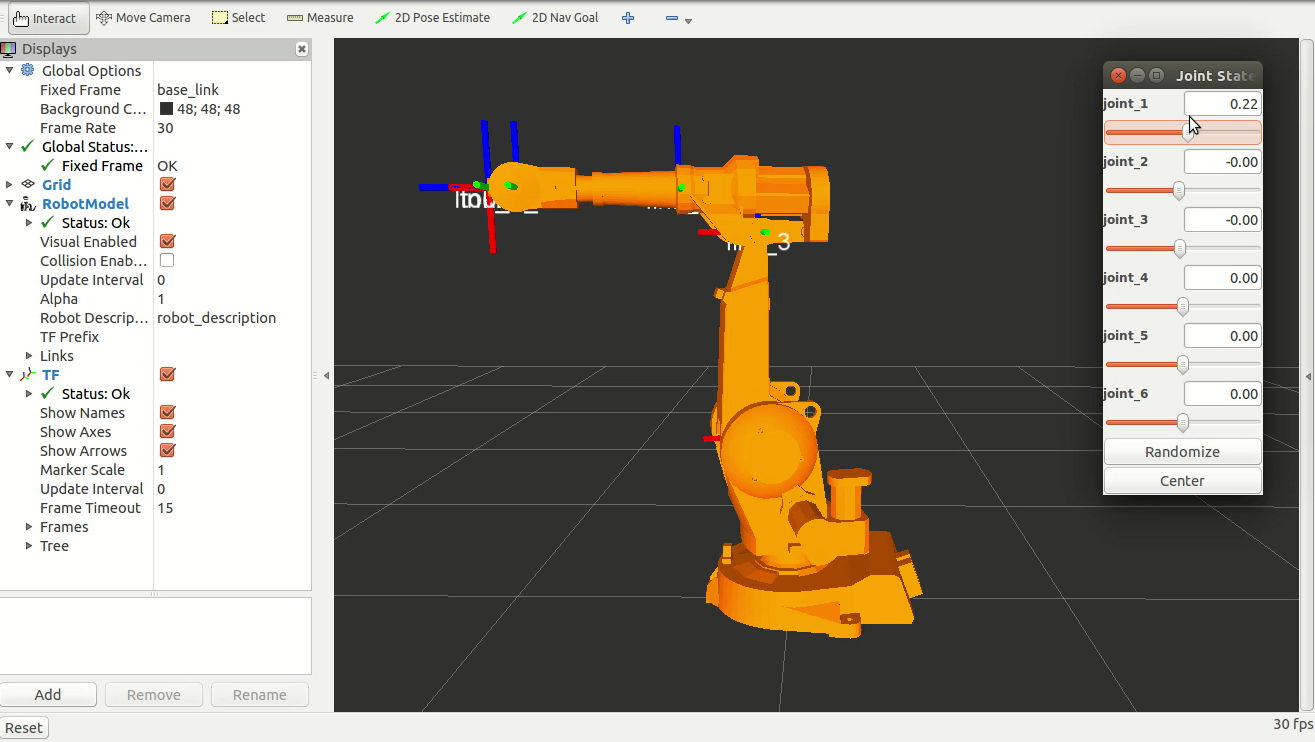
\includegraphics[width=0.8\linewidth]{Main/Chapter3/Images3/interfaz-rviz.png}
            \caption{ABB IRB 2400 con publicador de estado de juntas en RViz \cite{lentin_20188}}
            \label{f:Cap3-6_interfaz_rviz}
        \end{figure}
        
        \newpage
    
    \subsection{Coordenadas TF}
    
        Un marco de coordenadas o frame es un concepto importante en ROS. Cualquier robot puede tener varios componentes, como un láser, una cámara, un sonar o brazos, y pueden tener un marco de coordenadas adjunto. Muchos algoritmos ROS requieren realizar un seguimiento de todos estos marcos de coordenadas.
        
        TF son las siglas en ingles de marco de transformadas (Transform frames) y es una de las librerías fundamentales de ROS. TF está diseñada para proporcionar una forma estándar de realizar un seguimiento de los marcos de coordenadas y transformar los datos dentro de todo el sistema a lo largo del tiempo. El paquete TF puede rastrear y mantener la relación entre múltiples marcos de coordenadas. Su función es proporcionar herramientas y funciones para definir todos los marcos de coordenadas de nuestro robot y transformar datos de un marco a otro, como por ejemplo puntos o vectores.
        
        \begin{figure}[htb]
            \centering
            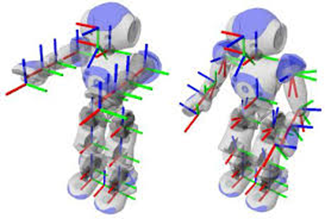
\includegraphics[width=1.0\linewidth]{Main/Chapter3/Images3/3-6/ejemplo-multiples-frames-rviz.png}
            \caption{Tres visualizaciones diferentes del modelo Minibot URDF. Visualizacion en Rviz, modelo de coliciones y estructura tf  \cite{phdthesistfhuman}. }
            \label{f:Cap3-6_frames_rviz}
        \end{figure}
        
Un ejemplo para explicar las coordenadas tf es el del robot simple  mostrado en la figura \ref{f:Cap3-6_nose1}, que tiene una base móvil con un láser montado encima. El objetivo de este robot es evitar obstáculos para no colisionar, como una pared.
En referencia al robot, se definen dos marcos de coordenadas: uno correspondiente al punto central de la base del robot llamado ''base\_link''y otro para el punto central del láser que está montado en la parte superior de la base movil llamado ''base\_laser''. 

El láser recopila datos en forma de distancias desde el punto central del láser a una pared, es decir, el láser tiene datos de distancia en el marco de coordenadas ''base\_laser''. Para evitar obstáculos se debe mover la base móvil, por los que los datos del láser se deben transformar al sistema de referencia ''base\_link'', en otras palabras,  se tiene que definir una relación entre los marcos de coordenadas ''base\_laser'' y ''base\_link''.
 \newpage
 
        \begin{figure}[htb]
            \centering
            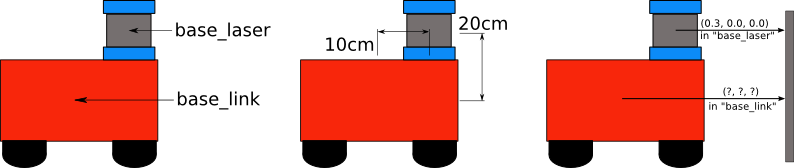
\includegraphics[width=1.0\linewidth]{Main/Chapter3/Images3/simple_robot.png}
            \caption{Ejemplo robot simple compuesto por base móvil y un láser}
            \label{f:Cap3-6_nose1}
        \end{figure}    

Esta relación entre los marcos de referencia son desplazamiento de traslación y rotacional entre los marcos 'base\_laser'' y ''base\_link''. Gestionar esta relación en todo momento en una simulación del robot , es decir, almacenar y aplicar los desplazamientos adecuados entre los fotogramas en cada momento, se convierte en un verdadero problema a medida que aumenta el número de fotogramas de coordenadas. Afortunadamente, sin embargo, no se tiene que hacer este trabajo ya que en su lugar, se define la relación entre "base\_link" y "base\_laser" una sola vez usando tf y la bibloteca tf gestiona la transformación entre los dos marcos de coordenadas automáticamente.

Para definir y almacenar la relación entre los marcos ''base\_link'' y ''base\_laser'' usando tf, se necesita crear a un árbol de transformación. Conceptualmente, cada nodo en el árbol de transformación corresponde a un marco de coordenadas y cada borde corresponde a la transformación que debe aplicarse para pasar del nodo actual a su hijo. Tf usa una estructura de árbol para garantizar que haya un solo recorrido que vincule dos marcos de coordenadas cualesquiera, y asume que todos los bordes del árbol se dirigen desde los nodos principales a los secundarios.    


        \begin{figure}[htb]
            \centering
            \includegraphics[width=1.0\linewidth]{Main/Chapter3/Images3/tf_robot.png}
            \caption{Láser recolectando datos respecto a ''base\_laser'', árbol de transformación y datos del láser transformados a marco ''base\_link'' }
            \label{f:Cap3-6_nose1}
        \end{figure}    
        
        
         TF ofrece una serie de herramientas o aplicaciones que facilitan al usuario la visualización del estado de las transformadas como:
        
        \begin{itemize}
            \item \textbf{tf\_monitor:} Imprime la información sobre el árbol de transformación actual.
            \item \textbf{tf\_echo:} Imprime información sobre la transformación entre dos fotogramas.
            \item \textbf{tf\_tree:} Crea un gráfico visual del árbol de transformación (en formato pdf).
        \end{itemize}
        
        \newpage
        La figura \ref{f:Cap3-6_sistema_arbol_tf} muestra un ejemplo de un árbol de transformada haciendo uso de la herramienta rqt\_tf\_tree y la figura \ref{f:Cap3-6_NOSE_tf} los respectivos marcos de referencia de cada parte del robot . En las dos figuras se puede observar los distintos frames del sistema y sus relaciones.
        
        \begin{figure}[htb]
            \centering
            \includegraphics[width=0.7\linewidth]{Main/Chapter3/Images3/3-6/ejemplo-frames-sistema-arbol.png}
            \caption{Frames de un sistema visualizado mediante tf\_tree}
            \label{f:Cap3-6_sistema_arbol_tf}
        \end{figure} 
        
        
        \begin{figure}[htb]
            \centering
            \includegraphics[width=0.55\linewidth]{Main/Chapter3/Images3/3-6/nose2.png}
            \caption{Figura que contiene los marcos tf más utilizados \cite{10.5555/2904061}}
            \label{f:Cap3-6_NOSE_tf}
        \end{figure} 
        
    
        Resumiendo esta sección, TF es una biblioteca con las siguientes características:
        
        \begin{itemize}
            \item Es una herramienta para realizar un seguimiento de los marcos de coordenadas a lo largo del tiempo.
            \item Mantiene la relación entre los marcos de coordenadas en una estructura de árbol almacenada en el tiempo
            \item Permite al usuario transformar puntos y vectores entre marcos de coordenadas en cualquier momento deseado
            \item Es implementado como modelo de publisher/subscriber en los temas con nombres /tf y /tf\_statics
        \end{itemize}
        
                        \newpage

    \subsection{Unified Robot Description Format (URDF)}\label{cap2_urfdf}
    
        \subsubsection{Introducción URDF}
    
        En ROS, es posible visualizar un modelo de un robot mediante el uso de archivos de formato de descripción de robot unificado (URDF). Sin embargo, solo aquellos robots que tienen eslabones rígidos conectados mediante articulaciones pueden ser descritos mediante modelos URDF.  Se puede usar un modelo URDF para calcular la cinemática, agregar nuevos marcos de coordenadas y moverlos de acuerdo con los valores del codificador del robot. Además, puede incluir otras propiedades físicas como inercia, colisiones, dinámica de articulaciones, etc. 
        
        Los archivos URDF están basados en XML y como tal, están compuestos por etiquetas de XML especiales que pueden ser leídas para extracción de información. A la lectura del archivo para extraer la información importante del modelo se denomina parsing y al programa o función que lo realiza, parser.
        
        La descripción del modelo consiste básicamente en de unir dos conjuntos: el conjunto de enlaces (link) y el conjunto de uniones (Joint). La forma de construir y visualizar un modelo de robot en URDF es escribir y compilar el archivo URDF. Una vez que se crea la representación 3D de un robot mediante el uso de un archivo URDF, es posible utilizar dicha representación para simular el movimiento del robot. Para ello, el usuario debe publicar las condiciones del robot en TF, utilizando un nodo (o nodos) para publicar la información de transformación.
        
        \begin{figure}[htb]
            \centering
            \includegraphics[width=0.55\linewidth]{Main/Chapter3/Images3/3-7/representacion-de-eslabon-en-urdf.png}
            \caption{Elementos basicos de visualization URDF: links y joints \cite{urdftutorials}.}
            \label{f:Cap3-7_eslabon_urdf}
        \end{figure} 
        
                                \newpage

        
        \subsubsection{Links}
        
        Los eslabones o enlaces (conjunto link) describen la parte física rígida del robot y permite especificar sus propiedades, como tamaño, forma, color o una malla 3D compleja importada. Consta de tres elementos:
    
        \begin{figure}[htb]
            \centering
            \includegraphics[width=0.8\linewidth]{Main/Chapter3/Images3/3-7/eslabon2.png}
            \caption{Reparcelación de la visual, inercia y colisión de un link con sus respectivos marcos de referencia para urdf  \cite{urdftutorials}}
            \label{f:Cap3-7_noseee_urdf}
        \end{figure} 

        \begin{enumerate}
            \item \textbf{Inertial:} Especifica las propiedades inerciales del link (posición del centro de masas, la masa y la matriz Inercia)
            \item \textbf{Visual:} en este elemento viene especificado como debe estar representado el link. Es posible usar solidos simples como una esfera o un cilindro, o hacer representaciones más trabajadas como mallados o nube de puntos. Del mismo modo, también y se pueden definir los colores e importar texturas.
            \item \textbf{Collision:} Describe las propiedades de colisión de los links. Puede ser una forma diferente a la visual, como una figura más simple que sea representativa, a fin de reducir los tiempos de calculo en las simulaciones.
        \end{enumerate}
        
        \begin{figure}[htb]
            \centering
            \includegraphics[width=0.9\linewidth]{Main/Chapter3/Images3/3-7/codigo.png}
            \caption{Descripción de un link en código URDF}
            \label{f:Cap3-7_nose_nose}
        \end{figure} 
        
                                \newpage

        
        \subsubsection{Joints}
        
        Las articulaciones o uniones (conjunto joint) indican la relación entre los distintos eslabones del robot. Describen además la cinemática y dinámica de cada articulación, además de especificar los límites de colisión del robot. Una articulación queda fefinida cuando se especifican los eslabones que une: el primero es llamado el padre (parent) y el segundo el hijo (child).
        
        \begin{figure}[htb]
            \centering
            \includegraphics[width=0.65\linewidth]{Main/Chapter3/Images3/3-8/representacion-de-una-articulacion-en-URDF.png}
            \caption{Representación gráfica de un joint y su relación padre-hijo con los link \cite{urdftutorials}}
            \label{f:Cap3-8_nose_nose}
        \end{figure} 
        
        Tipos de articulaciones:
        
        \begin{enumerate}
           \item \textbf{Revolute:} Permite que dos sólidos giren alrededor de un eje común y tiene un giro limitado especificado por un límite superior y uno inferior.
            \item \textbf{Continuous:} Se trata de una articulación de Revolute pero sin límites..
            \item \textbf{Prismatic:} Una junta que se deslizarse a lo largo de un eje. Tiene un alcance acotado por un límite inferior y uno superior.
            \item \textbf{Fixed:} No es realmente una articulación porque impide el movimiento. La unión no tiene ningún grado de libertad. Este tipo de articulación no requiere de ninguno de los elementos que describe la articulación..
            \item \textbf{Floating:} Esta unión mantiene libres todos los grados de libertad..
            \item \textbf{Planar:} Articulación que permite el movimiento en un plano.
        \end{enumerate}
        
                                        \newpage

        
        \begin{figure}[htb]
            \centering
            \includegraphics[width=1.0\linewidth]{Main/Chapter3/Images3/3-8/codigo-joint.png}
            \caption{Descripción de un joint en código URDF}
            \label{f:Cap3-8_nose_nose}
        \end{figure} 
        
        Cada conjunto de uniones (joint) está compuesto por hasta nueve elementos:
        
         \begin{enumerate}      
            \item \textbf{Origin:} es la posición donde se encuentra la unión entre el sólido padre (Parent) y el sólido hijo (child), en referencia al primero.
            \item \textbf{Parent:} el objeto padre en una unión
            \item \textbf{Child:} en objeto hijo en una unión
            \item \textbf{Axis:} eje del articulacion en la referencia global.
            \item \textbf{Calibration:} es un elemento opcional. Sirve para determinar la posición absoluta de la articulación
            \item \textbf{Dynamics:} es un elemento opcional. Define la amortiguación y la fricción de la articulación.
            \item \textbf{Límite:} sólo obligatoria en las articulaciones de revolución y en las prismáticas. Define el límite inferior y superior de la articulación, el esfuerzo máximo que puede aplicar y la velocidad máxima de esta.
            \item \textbf{Mimic:} es un elemento opcional. Se usa para especificar que una articulación imita a otra articulación ya existente. 
            \item \textbf{Safety controller:} es un elemento opcional. Específica para qué valores debe empezar a limitar la posición o la velocidad de una articulación en función de los límites establecidos en el tag <límit>.
        \end{enumerate}
        
                                                \newpage

    \subsection{Herramientas complementarias}
    
        Algunos paquetes y herramientas utiles para la interaccion con modelos URDF son los siguientes:
      
        \begin{itemize}
            \item \textbf{Joint\_state\_Publisher:} Este paquete contiene un nodo del mismo nombre que lee la descripción del modelo del robot, encuentra todas las articulaciones (joints) y publica los valore articulares para todas las articulaciones movibles usando sliders.
            \item \textbf{robot\_state\_Publisher:} Este paquete lee el estado de las articulaciones del robot y publica las posiciones y orientaciones 3D de cada eslabón usando la cinemática obtenida a partir del URDF. La posición 3D del robot se publica como una transformación (tf) que define las relaciones entre los sistemas de coordenadas.
            \item \textbf{xacro:} Significa Xml mACROs y es un formato que permite utilizar variables y otros add-ons para la generación de modelos complejos en formato URDF. De esta forma los modelos pueden ser más fáciles de entender y más mantenibles.
        \end{itemize}      
        
        La herramienta urdf\_to\_graphiz sirve para para obtener un diagrama graphviz de su archivo urdf, tal como se aprecia en la figura \ref{f:Cap3-9_nose_nose}:
        
        \begin{figure}[htb]
            \centering
            \includegraphics[width=0.43\linewidth]{Main/Chapter3/Images3/3-9/Esquema-de-los-componentes-de-un-fichero-urdf.png}
            \caption{Ejemplo de la representación gráfica URDF de un robot por medio de la herramienta urdf\_to\_graphiz \cite{urdftutorials}}
            \label{f:Cap3-9_nose_nose}
        \end{figure} 
        
    \newpage

\section{ADAMS (Automated Dynamic Analysis of Mechanical Systems)}

    % Adams es el software de análisis de movimiento y dinámica multicuerpo más utilizado en el mundo. Adams ayuda a los ingenieros a estudiar la dinámica de las piezas móviles, cómo se distribuyen las cargas y fuerzas en los sistemas mecánicos y a mejorar y optimizar el rendimiento de sus productos. El software de dinámica multicuerpo de Adams permite a los ingenieros crear y probar fácilmente prototipos virtuales de sistemas mecánicos en una fracción del tiempo y el costo necesarios para la construcción y prueba físicas. A diferencia de la mayoría de las herramientas integradas de CAD, Adams incorpora la física real resolviendo simultáneamente ecuaciones de cinemática, estática, cuasi-estática y dinámica. Al utilizar la tecnología de solución de dinámica multicuerpo, Adams también ejecuta dinámica no lineal en una pequeña fracción del tiempo requerido por las soluciones FEA. Las cargas y fuerzas calculadas por las simulaciones de Adams mejoran la precisión de FEA al proporcionar una mejor evaluación de cómo varían en una amplia gama de entornos operativos y de movimiento.

    Adams es un programa para simulación dinámica y análisis de movimiento cinemático en múltiples cuerpos. Ayuda en el estudio de la dinámica de las partes móviles, como cargas y fuerzas que se distribuyen a lo largo de los sistemas mecánicos, para mejorar y optimizar el rendimiento de los productos. Permite  crear y probar prototipos virtuales de los sistemas mecánicos en una fracción del tiempo y costo requerido para la estructura física y la prueba, incorporando la física real de forma simultánea a la resolución de ecuaciones de cinemática, estática, y la dinámica.

    Adams ejecuta la dinámica no lineal en una fracción del tiempo requerido por las soluciones de FEA. Proporcionando una mejor evaluación de la forma en que varían a través de una gama completa de movimiento y entornos operativos.
    
    Los módulos opcionales e integrados con Adams permiten a los usuarios integrar los componentes mecánicos, neumática, hidráulica, electrónica y tecnologías de control de sistemas para construir y probar prototipos virtuales que representan con precisión las interacciones entre estos subsistemas.


    \subsection{Análisis de sistemas multicuerpo}
    
    Un sistema multicuerpo es la modelización de un sistema mecánico como un conjunto de sólidos rígidos o flexibles conectados entre sí por un conjunto de uniones. Este conjunto forma un sistema físico cuya cinemática y dinámica se pueden describir con una serie de ecuaciones diferenciales y algebraicas
    
    \subsection{Descripción del ambiente de ADAMS}
    
    
    


% COPY PASTE DE VARIOS PAPEOS, PARA POSTERIOR MEJORA Y INTRODUCCIÓN AL CONTEXTO DE NUESTRA TESIS

    % La simulación de sistemas robotizados esta íntimamente ligada a la potencia
    % computacional de los procesadores de cálculo. El gran avance producido
    % con los microprocesadores actuales, ha permitido el desarrollo de diferentes
    % paquetes de simulación dinámica capaces de simular el comportamiento dinámico
    % de casi cualquier mecanismo multicuerpo. En esta tesis, el modelo del robot delta en estudio es construido en ADAMS.
    
    


    

    
    
    \begin{figure}[htb]
        \centering
        \includegraphics[width=1\linewidth]{Main/Chapter3/Images3/adams/logo_adams.png}
        \caption{Iamgen de referencia del software Adams}
        \label{f:Cap3-adams_logo}
    \end{figure} 
    

    
      
        
            
            
            

        
    
    